\documentclass[11pt,a4paper]{article}
\usepackage[T1]{fontenc}
\usepackage[utf8]{inputenc}
\usepackage{amsmath,amssymb,amsthm,mathtools}
\usepackage{geometry}
\usepackage{microtype}
\usepackage{lmodern}
\usepackage{tikz}
\usetikzlibrary{positioning,arrows.meta,calc,shapes,fit,backgrounds}
\usepackage{pgfplots}
\pgfplotsset{compat=1.18}
\usepackage{graphicx}
\usepackage[hidelinks]{hyperref}
\geometry{margin=2.5cm}

\theoremstyle{definition}
\newtheorem{definition}{Definition}[section]
\theoremstyle{plain}
\newtheorem{theorem}{Theorem}[section]
\newtheorem{lemma}[theorem]{Lemma}
\newtheorem{proposition}[theorem]{Proposition}
\newtheorem{corollary}[theorem]{Corollary}
\theoremstyle{remark}
\newtheorem{remark}[theorem]{Remark}
\newtheorem{example}[theorem]{Example}

\DeclareMathOperator{\Tr}{Tr}
\DeclareMathOperator{\Herm}{Herm}
\DeclareMathOperator{\rad}{rad}
\DeclareMathOperator{\diam}{diam}
\DeclareMathOperator{\embdim}{embdim}
\newcommand{\Lin}{\mathcal L}
\newcommand{\Chan}{\mathbf{Chan}}
\newcommand{\UChan}{\mathbf{UChan}}
\newcommand{\Sstate}{\mathcal{S}}
\newcommand{\TPHP}{\mathbf{TP}_{\mathrm{HP}}}
\newcommand{\rhodep}{\rho_{\mathrm{dep}}}
\newcommand{\id}{\mathrm{id}}
\newcommand{\affdim}{\dim_{\mathrm{aff}}}

\title{Exact Diamond Balls, Antipodal Widths, and Query-Uniform Compression Bounds for Quantum Channels}
\author{Amin Abaee\\
\small Independent Researcher\\
\small ORCID: 0000-0002-0019-1842\\
\small Email: \href{mailto:amin\_abaee@ut.ac.ir}{amin\_abaee@ut.ac.ir}}
\date{September 14, 2026}

\begin{document}
\maketitle

\begin{abstract}
Quantum channels with fixed finite-dimensional input and output form a compact convex body. We ask how many continuous latent parameters are needed to encode an arbitrary channel and reconstruct it with uniformly small diamond-norm error, when the encoder is continuous and the decoder is unrestricted. This is a continuous analogue of nonlinear width, distinct from tomography, which counts channel uses, and from programmable processors, which fix a decoding device. For a compact source the optimal error equals the minimal worst-case radius of the encoder's fibers. Lower bounds follow from antipodal pairs in the source and from latent collision topology via Borsuk--Ulam and the deleted-product coindex. Even input-independent output preparation forces error one below the output-state dimension, with a Clifford analogue inside the unitary channels. We determine the largest diamond ball contained in the channel body: it is centred at the completely depolarizing channel, is optimal among all centres, and, together with a full-direction section, certifies the intermediate lower envelope; the same channel is the optimal constant decoder, with exact covering radius, so the two envelopes meet at the exact width at zero latent dimension. Constructive upper bounds from convex projection and balanced pinching bracket the intermediate widths, and meet the lower envelope in the degenerate collapse case and from the affine dimension on. Every finite-query adaptive network induces a continuous final code containing all side information, so the same bottlenecks hold uniformly in the number of queries, for uniformly successful postselection, and for sampled transcripts; a one-query informationally complete measurement achieves the injective threshold, and repetition gives an $O(N^{-1/2})$ expected-error bound. In the input-independent case the widths are governed by the companion's flatness dichotomy: the flat value one fails for every output dimension at least three at the bottom two latent dimensions, the qutrit sitting exactly at $4/3$ there, through a flag-quotient cohomology computation.
\end{abstract}

\noindent\textbf{Keywords:} quantum channel compression; diamond norm; antipodal width; exact in-radius; nonlinear approximation; Borsuk--Ulam theorem.

\section{Introduction}

For fixed finite-dimensional input and output systems, quantum channels form
a compact convex body. The question is whether this body admits a continuous
low-dimensional encoding with uniformly accurate reconstruction in diamond
norm.

The problem differs from tomography and programming. Tomography asks how
many uses of an unknown channel are needed to produce an estimator. A
programmable processor uses a fixed physical device to transform a program
state into an implemented channel~\cite{NielsenChuang1997}. Here continuity
is imposed on the encoder, while the decoder is initially unrestricted. The
problem is therefore an encoder--decoder variant of continuous nonlinear
approximation~\cite{DeVoreHowardMicchelli1989}. Stable manifold methods and
Lipschitz widths provide related regularity-sensitive benchmarks
\cite{CohenEtAl2022,PetrovaWojtaszczyk2023}, while topological limitations of
autoencoding are studied in
\cite{BatsonEtAl2021,KvalheimSontag2024}. Variational quantum-circuit
autoencoders give an architecture-specific channel-compression model
\cite{WuEtAl2024}; the bounds here instead range over every continuous encoder
with the stated latent type.

Query complexity and retained representation dimension are different
resources: more channel uses may improve tomography, while a fixed
low-dimensional continuous code can remain topologically unable to represent
the full channel body. Related distinctions between query and memory
resources occur in quantum process learning~\cite{Caro2024}. Encoder
continuity is an explicit representational hypothesis, not a claim about
every possible synthesis map. Deterministic finite-query networks provide a
broad physical class for which this hypothesis follows from a proved
Lipschitz estimate. Robustness to perturbations of the stored code is a
separate decoder-regularity question.

The abstract theory separates three objects. First, unrestricted decoding
allows an exact fiber-radius characterization of reconstruction width.
Second, an antipodal separation profile measures the metric size of spherical
sections in the source. Third, the $\mathbb Z_2$-coindex of the deleted
product of a latent space determines which spherical maps must have an
antipodal collision. Euclidean Borsuk--Ulam is recovered as the basic case.

The channel application has two geometric scales. The full output-state
space, embedded by replacement channels, gives perfect antipodal separation
through index $d_B^2-2$. Across every remaining subcritical affine dimension,
the exact depolarizing-centred ball gives the lower bound
$2/[d_B\min\{d_A,d_B\}]$. Conversely, affine projection gives a universal
upper envelope near the affine threshold, while physical input/output
pinching retains selected coherent sectors and gives stronger structured
upper bounds at lower dimensions. Structured block joins are retained in
the appendix, and anticommuting Clifford generators give a perfectly
separated sphere inside the unitary channels for every square system of
dimension at least two.

A deterministic finite adaptive network, equivalently a finite quantum comb~\cite{Chiribella2009} and quantum strategy~\cite{GutoskiWatrous2007}, produces a continuous final code. Every quantum or
classical register available to reconstruction is part of that code. The
result applies to every finite query count and to uniformly successful
postselection on the channel domain under consideration, but not to
conditioning on events whose probability can vanish. The unrestricted
state-space decoder is distinguished from a fixed physical programmable
processor.

The contributions are: (i) an exact fiber-radius characterization of encoder-continuous width with unrestricted decoder; (ii) a source--latent collision theorem via antipodal profile and deleted-product coindex, recovering Euclidean Borsuk--Ulam as a special case; (iii) a maximal metric lower bound $1$ through index $L_{A,B}$ from the replacement family, the observable sphere, and their join, a full-direction section certifying $1/d_A$ through the affine dimension, and a Clifford unitary analogue; (iv) the exact all-dimensional depolarizing-centred in-radius --- optimal among all centres --- and the exact Chebyshev covering radius, with variational and spectral certificates; (v) constructive upper envelopes from convex projection and balanced input/output pinching, bracketing the widths below the affine threshold; (vi) query-uniform final-code bottlenecks for deterministic finite-query combs, uniformly successful postselection, and finite sampled transcripts, together with a one-query injective encoding and $O(N^{-1/2})$ finite-sample upper bound. The exact positive widths below the affine dimension remain open.

Section~\ref{sec:source-latent} develops fiber radii, antipodal profiles, and
latent-space collisions. Section~\ref{sec:geometry} then fixes the channel
and norm conventions used in the applications. Section~\ref{sec:balls}
studies relative diamond balls and centred in-radii.
Section~\ref{sec:replacement-unitary} develops the replacement, observable,
full-direction, and Clifford sections and the resulting channel lower and constructive upper envelopes. Section~\ref{sec:codes}
treats abstract state alphabets and physical programs.
Section~\ref{sec:adaptive} gives the adaptive-network consequences, and
Section~\ref{sec:conclusion} records scope and open questions. The appendix
collects the longer proofs of the radius and covering results, fixed-marginal
twirling, programming packing, structured partitions, and the Clifford
construction. Ref.~\cite{CompanionInstruments} extends the ball and compression theorems to finite-outcome quantum instruments and records, in an appendix, the no-programming background including the mixed-program and unequal-output cases; conversely, the channel-level theorems of the present paper are recovered from the instrument results by taking $n=1$.

Throughout, all systems are finite-dimensional and all latent dimensions are
real dimensions. Unless stated otherwise, the encoder is continuous and the
decoder has no regularity requirement. The complete retained code is defined as the density operator, classical probability law, sampled symbol, or
classical--quantum state containing all registers, outcomes, and side
information available at reconstruction time before decoding; every classical transcript, quantum register, reference system, or side register available to the decoder is part of the code. An averaged (deterministic) code state is distinguished from a single-run sampled transcript. The diamond norm uses a
reference system of input dimension $d_A$.

\section{Source--latent obstructions}
\label{sec:source-latent}

Let $K$ be a compact subset of a metric space $(X,d)$. The decoder target
$X$ may equal $K$ or may be a larger ambient metric space.

\subsection{Fiber radii and antipodal profiles}

\begin{definition}[Encoder-continuous reconstruction width]
\label{def:width}
For a topological latent space $Y$, define
\[
\delta^{\mathrm c}(K;Y,X)
:=
\inf_{\substack{f:K\to Y\ \mathrm{continuous}\\g:Y\to X}}
\sup_{x\in K}d(g(f(x)),x).
\]
For $Y=\mathbb R^r$, write $\delta_r^{\mathrm c}(K;X)$, with
$\mathbb R^0$ a singleton. No regularity is imposed on $g$. If no continuous $f:K\to Y$ exists (e.g., $K$ nonempty and $Y$ empty), define the infimum over an empty set to be $+\infty$.
\end{definition}

This is a variant of continuous nonlinear width in which only the encoder is
required to be continuous. We refer to this quantity as the compression
width.

\begin{definition}[Fiber radii and fiber diameter]
\label{def:fiber-widths}
For nonempty $F\subseteq K$, set
\[
\rad_X(F)=\inf_{z\in X}\sup_{x\in F}d(z,x).
\]
For a topological latent space $Y$, define
\[
\nu(K;Y,X)
=\inf_{f\in C(K,Y)}
  \sup_{y\in f(K)}\rad_X(f^{-1}(y)).
\]
For $Y=\mathbb R^r$, write $\nu_r(K;X)$. Also define
\[
\mu_r(K)
=\frac12\inf_{f\in C(K,\mathbb R^r)}
  \sup_{y\in f(K)}\diam f^{-1}(y).
\]
\end{definition}

\begin{theorem}[Exact fiber-radius characterization]
\label{thm:fiber-radius}
For every topological latent space $Y$,
\[
\delta^{\mathrm c}(K;Y,X)=\nu(K;Y,X).
\]
In particular, for every $r\in\mathbb N_0$,
\[
\delta_r^{\mathrm c}(K;X)=\nu_r(K;X),
\qquad
\mu_r(K)
\leq\delta_r^{\mathrm c}(K;X)
\leq2\mu_r(K).
\]
\end{theorem}

\begin{proof}
Fix $f\in C(K,Y)$. A decoder value $g(y)$ affects only the fiber
$f^{-1}(y)$, so its least possible worst error on that fiber is
$\rad_X(f^{-1}(y))$. Thus every decoder has error at least the supremum of
the fiber radii. Conversely, for every $\varepsilon>0$ and every
$y\in f(K)$, choose $z_y\in X$ such that
\[
\sup_{x\in f^{-1}(y)}d(z_y,x)
\leq\rad_X(f^{-1}(y))+\varepsilon.
\]
Define $g(y)=z_y$ on $f(K)$ and define it arbitrarily on $Y\setminus f(K)$.
No compatibility between these choices is required because the decoder has
no regularity assumption. The resulting error is at most the supremum of
the fiber radii plus $\varepsilon$. Letting $\varepsilon\downarrow0$ and
then taking the infimum over $f$ proves the identity. If $X$ is compact,
the radius function
$z\mapsto\sup_{x\in F}d(z,x)$ is $1$-Lipschitz, hence continuous, since
$|\sup_{x\in F}d(z,x)-\sup_{x\in F}d(z',x)|\le d(z,z')$, and therefore attains its infimum on $X$ for every
nonempty $F\subseteq K$. The same conclusion holds when $X$ is proper:
$F$ is bounded because $F\subseteq K$, and the centre search may be
restricted to a sufficiently large compact ball (closed balls are compact in a proper metric space). In either case the
$\varepsilon$-selection is unnecessary.

For every nonempty $F\subseteq K\subseteq X$,
\[
\frac12\diam F\leq\rad_X(F)\leq\diam F.
\]
The first inequality is the triangle inequality. For the second, choose a
point of $F$ as centre. Taking the relevant suprema and infima gives the
factor-two comparison.
\end{proof}

\begin{remark}[Fiber picture]
The encoder $f$ partitions $K$ into fibers $f^{-1}(y)$. For fixed $f$, the decoder value $g(y)$ can be optimized independently for each fiber because no regularity is imposed on $g$; the optimal worst-case error on the fiber is its radius $\rad_X$. The width $\nu(K;Y,X)$ is therefore the minimal possible maximal fiber radius achievable by a continuous $f$.
\end{remark}

\begin{definition}[Antipodal separation profile]
\label{def:profile}
For $r\in\mathbb N_0$, define
\[
\alpha_r(K)
=\frac12\sup_{h\in C(S^r,K)}
\min_{u\in S^r}d(h(u),h(-u)).
\]
The minimum exists by compactness of $S^r$. The quantity $\alpha_r(K)$
is henceforth abbreviated to the antipodal profile.
\end{definition}

\begin{proposition}[Profile properties]
\label{prop:profile-properties}
Let $K$ be a compact metric space. In items involving a subspace
$F\subseteq K$, assume that $F$ is compact and carries the restricted
metric. Then the following hold.
\begin{enumerate}
\item $\alpha_{r+1}(K)\leq\alpha_r(K)$.
\item If $F\subseteq K$, then $\alpha_r(F)\leq\alpha_r(K)$.
\item If $F$ is compact, $T:F\to K$ is continuous and
$d(Tx,Ty)\geq c\,d(x,y)$ with $c\ge0$, then
$\alpha_r(K)\geq c\alpha_r(F)$.
\item $0\leq\alpha_r(K)\leq\diam(K)/2$.
\item If two metrics $d_0,d_1$ on $K$ induce the same topology (as any two norm-induced metrics on a finite-dimensional ambient space do) and satisfy
$|d_0(x,y)-d_1(x,y)|\leq\varepsilon$ uniformly on $K^2$, then
$|\alpha_r(K,d_0)-\alpha_r(K,d_1)|\leq\varepsilon/2$. Uniform closeness alone does not suffice: the perturbation $d_1(x,y)=d_0(x,y)+\varepsilon$ for $x\ne y$ is a uniformly $\varepsilon$-close metric inducing the discrete topology, for which discontinuous antipodal selectors enter the supremum.
\end{enumerate}
\end{proposition}

\begin{proof}
Restricting a map on $S^{r+1}$ to an equatorial $S^r$ proves the first
claim. The second follows because maps into $F$ are maps into $K$. For the
third, compose each spherical map with $T$ and use the distance inequality.
For every spherical map, each antipodal separation lies between zero and
$\diam(K)$, which proves the fourth claim after taking the minimum, supremum,
and factor one half. For the fifth, the common topology makes $C(S^r,K)$ the same class of maps for both metrics; for every fixed $h$ in this common class,
\[
\left|\min_u d_0(h(u),h(-u))-
\min_u d_1(h(u),h(-u))\right|\leq\varepsilon.
\]
Taking suprema over the common class preserves this estimate, and the factor one half gives the stated bound.
\end{proof}

\begin{theorem}[Antipodal and fiber lower bounds]
\label{thm:profile-fiber}
For every $r$,
\[
\alpha_r(K)\leq\mu_r(K)
\leq\delta_r^{\mathrm c}(K;X)
\leq2\mu_r(K).
\]
In particular,
\[
\delta_r^{\mathrm c}(K;X)\geq\alpha_r(K).
\]
\end{theorem}

\begin{proof}
Fix $f\in C(K,\mathbb R^r)$ and $h\in C(S^r,K)$. Borsuk--Ulam
\cite{Matousek2003} gives $u$ with $f(h(u))=f(h(-u))$. Hence one fiber
has diameter at least
\[
d(h(u),h(-u))
\geq\min_v d(h(v),h(-v)).
\]
Take the supremum over $h$, then the infimum over $f$, and divide by two to
obtain $\alpha_r(K)\leq\mu_r(K)$. The remaining inequalities are
Theorem~\ref{thm:fiber-radius}.
\end{proof}

\subsection{Intrinsic topology of the latent space}

The deleted product supplies an intrinsic collision criterion for the latent
space, independent of a chosen Euclidean embedding.

\begin{definition}[Deleted-product coindex]
\label{def:coindex}
For a Hausdorff space $Y$, let
\[
F_2(Y)=\{(y_0,y_1)\in Y^2:y_0\neq y_1\},
\]
with involution $(y_0,y_1)\mapsto(y_1,y_0)$. Define
\[
\operatorname{coind}_{\mathbb Z_2}F_2(Y)
=\sup\{k\in\mathbb N_0:\text{there exists a continuous equivariant map }
S^k\to F_2(Y)\},
\]
where $S^k$ has the antipodal action. If $F_2(Y)=\varnothing$, the value is
defined to be $-1$; otherwise the displayed supremum is used and may be
$+\infty$. This is the standard sphere-map coindex convention; see, for
example,~\cite{Matousek2003}. When the acting group is clear, we
occasionally suppress the subscript $\mathbb Z_2$.
\end{definition}

\begin{remark}[Configuration-space intuition]
$F_2(Y)$ is the ordered configuration space of two distinct latent codes. An equivariant map $S^r\to F_2(Y)$ assigns to each $u$ a distinct pair of codes for $u$ and $-u$ continuously and respecting antipodal symmetry. If such a map does not exist, every continuous $f\circ h:S^r\to Y$ must identify some antipodal pair, forcing a collision. The coindex is the largest $r$ for which collision can be avoided.
\end{remark}

\begin{theorem}[Intrinsic latent-space obstruction]
\label{thm:intrinsic-latent}
Let $Y$ be Hausdorff. If
\[
r>\operatorname{coind}_{\mathbb Z_2}F_2(Y),
\]
then every continuous $f:K\to Y$ and every decoder $g:Y\to X$ satisfy
\[
\sup_{x\in K}d(g(f(x)),x)\geq\alpha_r(K).
\]
\end{theorem}

\begin{proof}
Fix $h:S^r\to K$. If $f(h(u))\neq f(h(-u))$ for every $u$, then
\[
u\longmapsto(f(h(u)),f(h(-u)))
\]
is an equivariant map from $S^r$ to $F_2(Y)$, contradicting the coindex
hypothesis. Thus an antipodal pair has one code. The triangle inequality
forces one reconstruction error to be at least half the pair separation.
Take the supremum over $h$. An empty latent space admits no encoder from
the nonempty source; by the convention in Definition~\ref{def:width} the
width is then $+\infty$, so no separate case arises.
\end{proof}

\begin{proposition}[Euclidean recovery]
\label{prop:euclidean-coindex}
If $Y$ admits a continuous injection into $\mathbb R^s$, then
\[
\operatorname{coind}_{\mathbb Z_2}F_2(Y)\leq s-1.
\]
Consequently every continuous encoder through $Y$ has error at least
$\alpha_s(K)$. More generally, if a compact metric space $K$ admits a
continuous injection into $\mathbb R^s$, then
$\alpha_r(K)=0$ for every $r\geq s$. If $Y$ is a convex body with
nonempty interior in $\mathbb R^s$, then equality holds in the coindex
bound.
\end{proposition}

\begin{proof}
If $s=0$, injectivity into $\mathbb R^0$ forces $Y$ to have at most one
point. Thus $F_2(Y)=\varnothing$ and its coindex is $-1=s-1$. Likewise,
any compact $K$ that injects into $\mathbb R^0$ is a singleton, so
$\alpha_r(K)=0$ for every $r\geq0$.

Assume $s\geq1$ and let $\iota:Y\to\mathbb R^s$ be injective. The
normalised difference map
\[
(y_0,y_1)\longmapsto
\frac{\iota(y_0)-\iota(y_1)}
     {\|\iota(y_0)-\iota(y_1)\|_2}
\]
is equivariant from $F_2(Y)$ to $S^{s-1}$. An equivariant map
$S^k\to S^{s-1}$ cannot exist for $k\geq s$ by Borsuk--Ulam. Hence the
coindex is at most $s-1$, and Theorem~\ref{thm:intrinsic-latent} applies
with $r=s$.

If $K$ admits a continuous injection $\kappa:K\to\mathbb R^s$ and
$r\geq s$, then, for every $h:S^r\to K$, the generalised Borsuk--Ulam theorem (equivalently the nonexistence of an equivariant map $S^r\to S^{s-1}$ for $r\ge s$) applied to $\kappa\circ h$ gives a point $u$ with
$\kappa(h(u))=\kappa(h(-u))$. Injectivity gives $h(u)=h(-u)$, so every
such map has minimum antipodal separation zero and $\alpha_r(K)=0$.

For a full-dimensional convex body with $s\geq1$, choose an interior point
$y_0$ and $\varepsilon>0$ such that $y_0\pm\varepsilon u$ remain in the
body for all $u\in S^{s-1}$. The map
$u\mapsto(y_0+\varepsilon u,y_0-\varepsilon u)$ is equivariant into the
deleted product, proving the reverse inequality. For $s=0$, such a body
is a singleton and equality was already shown.
\end{proof}

\subsection{Convex and stable certificates}

The preceding results reduce reconstruction lower bounds to source
separation and latent collisions. For convex sources, norm balls and their
lower-dimensional sections provide explicit lower certificates, while affine
projection and fiber centres provide a general upper construction. When the
decoder is Lipschitz rather than unrestricted, the residual separation
of the reachable latent image yields a quantitative stable form.

\begin{theorem}[Contained-ball profile]
\label{thm:bottleneck}
Let $K$ be a compact subset of a $D$-dimensional normed affine space,
with its induced metric, and suppose
$\overline B(x_0,\rho)\subseteq K$. Then
\[
\alpha_r(K)\geq\rho,
\qquad0\leq r<D.
\]
\end{theorem}

\begin{proof}
Choose an $(r+1)$-dimensional subspace $W$ of the direction space, equip it
with an auxiliary Euclidean norm, and let $S_E^r\subset W$ be its unit sphere; write
$\|\cdot\|_{\mathrm{amb}}$ for the ambient norm. The radial map
\[
h(u)=x_0+\rho\frac{u}{\|u\|_{\mathrm{amb}}}
\]
is continuous and satisfies
$\|h(u)-h(-u)\|_{\mathrm{amb}}=2\rho$. This map is
admissible in Definition~\ref{def:profile}, so
$\alpha_r(K)\geq\rho$.
\end{proof}

\begin{definition}[Sectional in-radius]
\label{def:sectional-radius}
Let $K$ lie in a finite-dimensional normed affine space with direction
space $V$. For $0\leq r<\dim V$, define
\[
R_r(K)=
\sup_{\substack{x_0\in K,\ W\subseteq V\\\dim W=r+1}}
\sup\{\rho\geq0:x_0+\{w\in W:\|w\|\leq\rho\}\subseteq K\}.
\]
\end{definition}

\begin{proposition}[Sectional-radius certificate]
\label{prop:sectional-radius}
For every compact $K$ in a finite-dimensional normed affine space,
\[
\alpha_r(K)\geq R_r(K).
\]
Thus sectional convex geometry supplies profile lower bounds, while more
general antipodal constructions, such as Clifford and join sections, need
not arise as boundaries of norm balls.
\end{proposition}

\begin{proof}
For every admissible centre, subspace, and radius in
Definition~\ref{def:sectional-radius}, apply the radial construction from
Theorem~\ref{thm:bottleneck} inside $W$. It produces an $S^r$ with
antipodal separation $2\rho$. Taking the two suprema proves the claim.
\end{proof}

\begin{proposition}[Convex-projection upper bound]
\label{prop:convex-projection-upper}
Let $K$ be a compact convex subset of a $D$-dimensional normed affine
space, with diameter $\diam K=\sup_{x,y\in K}\|x-y\|$. Then, for $0\leq r\leq D$,
\[
\delta_r^{\mathrm c}(K;K)
\leq
\frac{D-r}{D-r+1}\,\diam K.
\]
\end{proposition}

\begin{proof}
For $r=D$, affine coordinates give exact reconstruction. Assume
$0\leq r<D$, put $k=D-r$, choose affine coordinates on
$\operatorname{aff}K$, and project them onto their first $r$ components.
This gives a continuous encoder $f:K\to\mathbb R^r$. Every nonempty fiber
$F_y=f^{-1}(y)$ is compact and convex, has diameter at most $\diam K$, and
has affine dimension at most $k$. Write $d_y=\operatorname{diam}F_y$.

Fix such a fiber and set
$R_y=k\,d_y/(k+1)$. In the affine hull of $F_y$, consider the family
\[
\mathcal F_y
=\{F_y\}\cup\{\overline B(x,R_y):x\in F_y\}.
\]
Work in the normed affine space $\operatorname{aff}(F_y)$, of dimension at most $k$, and replace each ambient ball $\overline B(x,R_y)$ by its intersection with $\operatorname{aff}(F_y)$, which remains convex and becomes compact after intersecting with $F_y$. Every subfamily of at most $k+1$ members has nonempty intersection. Indeed,
if it consists of $m\leq k+1$ balls centred at
$x_1,\ldots,x_m\in F_y$, their barycentre $c=m^{-1}\sum_jx_j$ lies in
$F_y$ and satisfies
\[
\|c-x_i\|
\leq\frac1m\sum_{j\neq i}\|x_j-x_i\|
\leq\frac{m-1}{m}\,d_y
\leq R_y.
\]
If the subfamily also contains $F_y$, then it contains at most $k$ balls,
and the same barycentre belongs to $F_y$ and satisfies the same estimate.
The case of no balls is immediate.

Helly's theorem~\cite{Barvinok2002} for convex sets in $\mathbb R^k$ now gives that every finite subfamily of $\mathcal F_y$ has nonempty intersection. Since we may intersect each member with the compact set $F_y$, the family $\{F_y\}\cup\{F_y\cap\overline B(x,R_y):x\in F_y\}$ consists of compact sets with the finite-intersection property. Hence there exists
\[
c_y\in F_y\cap\bigcap_{x\in F_y}\overline B(x,R_y).
\]
Define the decoder by $g(y)=c_y$ on $f(K)$ and arbitrarily elsewhere. Then
\[
\|g(f(x))-x\|
\leq\frac{k}{k+1}d_{f(x)}
\leq\frac{D-r}{D-r+1}\diam K
\]
for every $x\in K$, which proves the claim.
\end{proof}

\begin{proposition}[Exact Euclidean-coordinate threshold]
\label{prop:euclidean-threshold}
Let $K$ be compact, let its affine hull have dimension $D$, and equip it
with the metric induced by a norm on that affine hull. Then
$\delta_r^{\mathrm c}(K;K)=0$ for $r\geq D$, and the exact decoder may be chosen continuous. If $K$ contains a positive
relative ball---that is, a ball of positive radius $\rho>0$ in the relative topology of its affine hull, i.e., some $\overline B(x_0,\rho)=\{x_0+w:\|w\|\le\rho\}\subseteq K$ with $w$ in the direction space of $\operatorname{aff}K$---then
\[
\delta_r^{\mathrm c}(K;K)=0
\quad\Longleftrightarrow\quad r\geq D.
\]
\end{proposition}

\begin{proof}
Affine coordinates $c$, padded by zeros, give a continuous injection into
$\mathbb R^r$ for $r\geq D$. The image $c(K)$ is compact and convex; the
Euclidean nearest-point projection $\Pi_C$ onto a nonempty closed convex set
is single-valued and $1$-Lipschitz, hence continuous, and the decoder
$g=c^{-1}\circ\Pi_C\circ(\text{coordinate projection})$ is exact and
continuous on the encoder image, extended arbitrarily elsewhere, which
gives width zero. If $K$ contains
$\overline B(x_0,\rho)$ with $\rho>0$, then for every $r<D$,
Theorems~\ref{thm:profile-fiber} and~\ref{thm:bottleneck} give
$\delta_r^{\mathrm c}(K;K)\geq\rho>0$. Thus the infimum cannot vanish
below $D$, proving the converse implication without assuming that an
infimizing encoder--decoder pair exists.
\end{proof}

\begin{theorem}[Stable source--latent obstruction]
\label{thm:stable-obstruction}
Let $f:K\to Y$ be continuous, where $Y$ is a metric space, and let
$g:Y\to X$ be $L$-Lipschitz. Then
\[
\sup_{x\in K}d(g(f(x)),x)
\geq\alpha_r(K)-L\alpha_r(f(K)),
\]
where $f(K)$ carries the metric induced from $Y$.
\end{theorem}

\begin{proof}
The set $f(K)$ is compact. Fix $h:S^r\to K$ and set
$a_h=\min_u d(h(u),h(-u))$. The map
$u\mapsto d_Y(f(h(u)),f(h(-u)))$ is continuous on the compact sphere, so
it has a minimizer $u_0$. By the definition of the profile of $f(K)$,
\[
d_Y(f(h(u_0)),f(h(-u_0)))
\leq2\alpha_r(f(K)).
\]
If $E$ is the worst reconstruction error, then by the definition of $a_h$,
the triangle inequality, and the Lipschitz property,
\begin{align*}
a_h
&\leq d(h(u_0),h(-u_0))\\
&\leq d(h(u_0),g(f(h(u_0))))
+d(g(f(h(u_0))),g(f(h(-u_0))))
+d(g(f(h(-u_0))),h(-u_0))\\
&\leq2E+L\,d_Y(f(h(u_0)),f(h(-u_0)))\\
&\leq2E+2L\alpha_r(f(K)).
\end{align*}
Taking the supremum over $h$ and dividing by two proves the claim.
\end{proof}

Figure~\ref{fig:dependency} summarises the roles of fiber optimization,
source separation, and latent collision topology.

\begin{figure}[t]
\centering
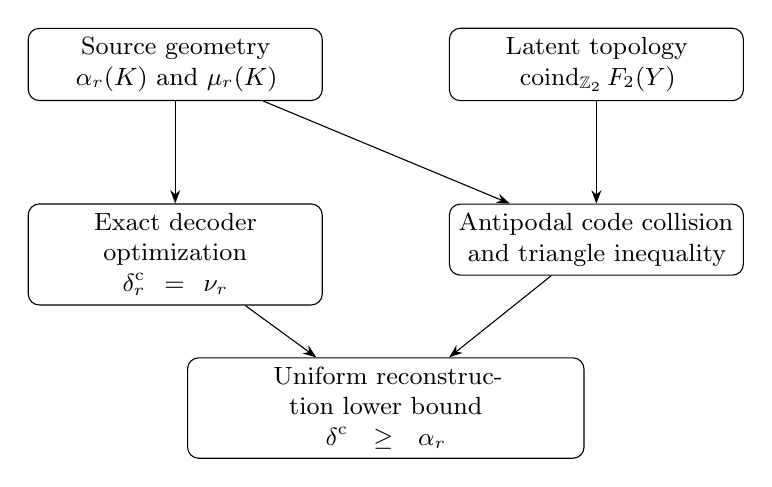
\begin{tikzpicture}[
  >=Stealth,
  box/.style={draw,rounded corners,align=center,minimum height=9mm,
              text width=35mm,font=\small},
  every node/.style={font=\small}
]
\node[box] (source) {Source geometry\\$\alpha_r(K)$ and $\mu_r(K)$};
\node[box,right=16mm of source] (latent) {Latent topology\\
$\operatorname{coind}_{\mathbb Z_2}F_2(Y)$};
\node[box,below=13mm of source] (fiber) {Exact decoder optimization\\
$\delta_r^{\mathrm c}=\nu_r$};
\node[box,below=13mm of latent] (collision) {Antipodal code collision\\
and triangle inequality};
\coordinate (midlower) at ($(fiber)!0.5!(collision)$);
\node[box,below=14mm of midlower,
      text width=48mm] (floor) {Uniform reconstruction lower bound\\
$\delta^{\mathrm c}\geq\alpha_r$};
\draw[->] (source) -- (collision);
\draw[->] (latent) -- (collision);
\draw[->] (source) -- (fiber);
\draw[->] (fiber) -- (floor);
\draw[->] (collision) -- (floor);
\end{tikzpicture}
\caption{Logical structure of the source--latent obstruction. Fiber radii
characterize unrestricted decoder optimization; antipodal source separation
and latent collision topology provide computable lower bounds.}
\label{fig:dependency}
\end{figure}


\section{Channel geometry and norm conventions}
\label{sec:geometry}

Let $A$ and $B$ be nonzero finite-dimensional Hilbert spaces, with
$d_A=\dim A$ and $d_B=\dim B$. Write $\Lin(A)$ for the linear operators on
$A$, and let $\Chan(A,B)$ denote the channels
$\Phi:\Lin(A)\to\Lin(B)$. Let $A_0\simeq A$ be a fixed reference copy and
set
\[
|\omega_A\rangle
=\frac1{\sqrt{d_A}}\sum_{j=1}^{d_A}|j\rangle_{A_0}|j\rangle_A.
\]
The normalised Choi operator of $\Phi$ is
\cite{Choi1975,Jamiolkowski1972}
\[
\widehat J_\Phi
=(\id_{A_0}\otimes\Phi)(|\omega_A\rangle\langle\omega_A|).
\]
Equivalently, with column vectorization
$|K\rangle\rangle=\sum_{a,b}K_{ba}|a\rangle_{A_0}|b\rangle_B$,
the unnormalized Choi operator of a completely positive map with Kraus
operators $K_\alpha$ is
$J_\Phi=\sum_\alpha|K_\alpha\rangle\rangle
\langle\langle K_\alpha|$.
Then
\[
\Phi\in\Chan(A,B)
\quad\Longleftrightarrow\quad
\widehat J_\Phi\geq0,
\qquad
\Tr_B\widehat J_\Phi=\frac{I_{A_0}}{d_A}.
\]
The affine direction space is
\[
V_{A,B}=\{X\in\Herm(A_0\otimes B):\Tr_BX=0\},
\]
so
\begin{equation}
\label{eq:channel-dimension}
D_{A,B}:=\affdim\Chan(A,B)=d_A^2(d_B^2-1).
\end{equation}
If $d_B=1$, the channel body is a singleton. Henceforth $d_B>1$.

The completely depolarizing channel is
\[
\Omega_{A,B}(X)=\Tr(X)\frac{I_B}{d_B},
\qquad
\widehat J_{\Omega_{A,B}}
=\frac{I_{A_0\otimes B}}{d_Ad_B}.
\]
Its Choi operator is positive definite, so it is a relative interior point; convex-geometric analyses of related quantum bodies are carried out in~\cite{SzarekBengtssonZyczkowski2006}.
For later use, the replacement channel associated with
$\sigma\in\Sstate(B)$ is
\[
\mathcal R_\sigma(X)=\Tr(X)\sigma.
\]

For a Hermiticity-preserving map
$\Delta:\Lin(A)\to\Lin(B)$,
\[
\|\Delta\|_\diamond
=
\sup_{\rho\in\Sstate(A_0\otimes A)}
\|(\id_{A_0}\otimes\Delta)(\rho)\|_1.
\]
A reference of dimension $d_A$ suffices~\cite{Watrous2018}. Operationally,
for two equally likely channels $\Phi$ and $\Psi$, the optimal single-use
discrimination error is
$\tfrac12-\tfrac14\|\Phi-\Psi\|_\diamond$, allowing arbitrary entangled
inputs and final measurements. Since the maximally entangled state is one
admissible input,
\begin{equation}
\label{eq:choi-diamond}
\|\widehat J_\Delta\|_1\leq\|\Delta\|_\diamond.
\end{equation}

\begin{lemma}[Trace-zero spectral bound]
\label{lem:trace-zero}
If $X=X^\dagger$ and $\Tr X=0$, then
\[
\|X\|_\infty\leq\frac12\|X\|_1.
\]
\end{lemma}

\begin{proof}
Write $X=X_+-X_-$ for its Jordan decomposition. Then
$X_\pm\geq0$, $X_+X_-=0$, and
$\Tr X_+=\Tr X_-=\|X\|_1/2$. For positive semidefinite $P$,
$\|P\|_\infty\leq\Tr P=\|P\|_1$. Hence
\[
\|X\|_\infty
=\max\{\|X_+\|_\infty,\|X_-\|_\infty\}
\leq\frac12\|X\|_1.
\]
\end{proof}

\begin{lemma}[Choi bounds in the present convention]
\label{lem:choi-upper}
Let $J_\Delta=d_A\widehat J_\Delta$ be the unnormalized Choi operator of
a Hermiticity-preserving map. Then
\[
\frac1{d_A}\|J_\Delta\|_1
\leq\|\Delta\|_\diamond
\leq\|\Tr_B|J_\Delta|\|_\infty.
\]
\end{lemma}

\begin{proof}
The lower bound is~\eqref{eq:choi-diamond}. For the upper bound, write the Jordan decomposition $J_\Delta=J_+-J_-$ with
$J_\pm\geq0$ of orthogonal support, and let $\Delta_\pm$ be the completely
positive maps with Choi operators $J_\pm$ (in the unnormalized convention
$J_\Delta=\sum_{i,j}|i\rangle\langle j|\otimes\Delta(|i\rangle\langle j|)$,
with trace over the output factor; the same bound for Hermiticity-preserving
maps is derived independently in~\cite[Corollary~2]{NechitaEtAl2018}).
For every state $\rho$ on a reference-and-input system,
$(\id\otimes\Delta)(\rho)=(\id\otimes\Delta_+)(\rho)-(\id\otimes\Delta_-)(\rho)$
is a difference of positive operators, so its trace norm is at most the sum
of their traces. Computing each trace through the adjoint gives
$\Tr[(\id\otimes\Delta_\pm)(\rho)]=\Tr[\rho\,(I\otimes\Tr_BJ_\pm)]$, so the
sum equals $\Tr[\rho\,(I\otimes\Tr_B|J_\Delta|)]$, which is at most
$\|\Tr_B|J_\Delta|\|_\infty$ because $\rho$ is a state. Taking the supremum
over $\rho$ proves the upper bound. We shall also use the elementary estimate
\[
\|\Tr_B|J_\Delta|\|_\infty
\leq\Tr(\Tr_B|J_\Delta|)
=\|J_\Delta\|_1,
\]
which follows because $\Tr_B|J_\Delta|$ is positive.
\end{proof}


\section{Relative diamond balls and centred in-radii}
\label{sec:balls}

The contained-ball profile theorem turns a channel-space in-radius into a
compression lower bound. This section therefore determines the largest
relative diamond ball about the completely depolarizing channel, first
stating the exact value and then isolating its spectral and variational
mechanisms.

A map $\Delta$ is trace-annihilating if $\Tr\Delta(X)=0$ for all $X$,
equivalently $\Tr_B\widehat J_\Delta=0$. Define
\[
\overline B^{\mathrm{rel}}_\diamond(\Phi_0,\rho)
=\{\Phi_0+\Delta:\Delta\text{ is Hermiticity-preserving and
trace-annihilating},\ \|\Delta\|_\diamond\leq\rho\}.
\]

\begin{definition}[Centered relative diamond in-radius]
For $\Phi_0\in\Chan(A,B)$, define
\[
\rho_\diamond(\Phi_0)
=\sup\{\rho\geq0:
\overline B^{\mathrm{rel}}_\diamond(\Phi_0,\rho)
\subseteq\Chan(A,B)\}.
\]
\end{definition}

\begin{definition}[Variational parameter]
Define
\[
\Gamma_{A,B}
=\sup\left\{
\lambda_{\max}(-\widehat J_\Delta):
\Delta\text{ is Hermiticity-preserving and trace-annihilating},\
\|\Delta\|_\diamond\leq1
\right\}.
\]
\end{definition}

\subsection{Exact centred radius}

\begin{theorem}[Exact depolarizing-centred in-radius]
\label{thm:exact-inradius}
Let
\[
s=\min\{d_A,d_B\}.
\]
Then
\[
\Gamma_{A,B}=\frac{s}{2d_A},
\qquad
\rho_\diamond(\Omega_{A,B})
=\rhodep(A,B)
:=\frac{2}{d_Bs}.
\]
Equivalently,
\[
\rho_\diamond(\Omega_{A,B})
=
\begin{cases}
2/(d_Ad_B),&d_A\leq d_B,\\[2pt]
2/d_B^2,&d_A>d_B.
\end{cases}
\]
\end{theorem}

The proof is given in Appendix~\ref{app:exact-inradius-proof}.

The exact theorem separates two dimension regimes. When $d_A\leq d_B$,
an isometric channel on the full input space is extremal. When $d_A>d_B$,
the extremal construction is supported on a $d_B$-dimensional input
subspace, and the radius ceases to depend on $d_A$. Operationally, the
relevant perturbation can be detected with a maximally entangled probe whose
Schmidt rank is at most
$s=\min\{d_A,d_B\}$. Extra input dimensions beyond the output capacity do
not produce a direction with a smaller positivity radius: the witness already
fits inside an output-sized input subspace. Thus $s$, rather than the full input
dimension alone, is the effective entanglement rank controlling robustness
of the completely noisy channel against arbitrary trace-preserving Hermitian
perturbations.

The following spectral certificate gives a direct but generally nonoptimal
contained ball; the variational formula then identifies the exact radial
optimization.

\subsection{Spectral and variational mechanisms}

\begin{proposition}[Centre-dependent spectral certificate]
\label{prop:spectral-centre}
Let $\Phi_0\in\Chan(A,B)$ have positive-definite normalised Choi operator
and set $\lambda_*=\lambda_{\min}(\widehat J_{\Phi_0})$. Then
\[
\overline B^{\mathrm{rel}}_\diamond(\Phi_0,2\lambda_*)
\subseteq\Chan(A,B).
\]
Among channel centres, the depolarizing channel uniquely maximises the
certificate $2\lambda_{\min}(\widehat J_{\Phi_0})$.
\end{proposition}

\begin{proof}
For an admissible perturbation $X=\widehat J_\Delta$,
Lemma~\ref{lem:trace-zero} and~\eqref{eq:choi-diamond} give
$\|X\|_\infty\leq\|\Delta\|_\diamond/2$. Thus
$\|\Delta\|_\diamond\leq2\lambda_*$ implies
$\widehat J_{\Phi_0}+X\geq0$; the marginal constraint is unchanged.

Every normalised Choi operator has trace one on a space of dimension
$d_Ad_B$, so $\lambda_*\leq1/(d_Ad_B)$. Equality forces every eigenvalue
to equal $1/(d_Ad_B)$, hence
$\widehat J_{\Phi_0}=I/(d_Ad_B)$ and $\Phi_0=\Omega_{A,B}$.
\end{proof}

At the depolarizing centre, Proposition~\ref{prop:spectral-centre} gives the
explicit certificate
\[
\overline B^{\mathrm{rel}}_\diamond
\left(\Omega_{A,B},\frac{2}{d_Ad_B}\right)
\subseteq\Chan(A,B),
\]
because $\widehat J_{\Omega_{A,B}}=I/(d_Ad_B)$. This certificate equals the
true centred radius when $d_A\leq d_B$ and is strictly smaller when
$d_A>d_B$.

\begin{proposition}[Variational formula for the centred in-radius]
\label{prop:inradius-variational}
The parameter $\Gamma_{A,B}$ satisfies
\[
\rho_\diamond(\Omega_{A,B})
=\frac{1}{d_Ad_B\,\Gamma_{A,B}}.
\]
Moreover, $0<\Gamma_{A,B}\leq1/2$.
\end{proposition}

\begin{proof}
Let $N=d_Ad_B$ and let $\mathcal D$ be the diamond unit sphere in the
finite-dimensional real vector space of Hermiticity-preserving,
trace-annihilating maps. The set $\mathcal D$ is compact. For
$\Delta\in\mathcal D$, put $X=\widehat J_\Delta$. The operator $X$ is
nonzero, Hermitian, and traceless, so
$\lambda_{\max}(-X)>0$. Along the ray
$\Omega_{A,B}+t\Delta$, complete positivity is equivalent to
\[
\frac IN+tX\geq0.
\]
The first boundary point occurs at
\[
t_\Delta=\frac{1}{N\lambda_{\max}(-X)}.
\]
Every nonzero affine perturbation has a unique representation as a positive
multiple of an element of $\mathcal D$, and every ray from the relative
interior point $\Omega_{A,B}$ meets the relative boundary before leaving the
channel body. Consequently,
\[
\rho_\diamond(\Omega_{A,B})
=\min_{\Delta\in\mathcal D}t_\Delta
=\frac{1}{N\max_{\Delta\in\mathcal D}
\lambda_{\max}(-\widehat J_\Delta)}.
\]
Continuity on the compact set $\mathcal D$ gives attainment and the displayed
formula for $\Gamma_{A,B}$.

Lemma~\ref{lem:trace-zero} and~\eqref{eq:choi-diamond} give
\[
\lambda_{\max}(-X)
\leq\frac12\|X\|_1
\leq\frac12\|\Delta\|_\diamond,
\]
so $\Gamma_{A,B}\leq1/2$. Positivity follows from any nonzero admissible
direction, after reversing its sign if necessary.
\end{proof}

\begin{remark}[Effective Schmidt rank]
The parameter $s=\min\{d_A,d_B\}$ is the largest Schmidt rank that can be supported simultaneously by input and output. The extremal perturbation is detected by a maximally entangled probe of rank $s$ supported on an $s$-dimensional input subspace $S_A\subseteq A$; the witness $V_0,V_1:S_A\to B$ with ${\rm Tr}V_0^\dagger V_1=0$ of the appendix proof uses only this subspace. Extra input dimensions beyond output capacity do not reduce the radius.
\end{remark}

\subsection{Benchmark distance}

For square systems, the identity channel gives a convenient normalisation
check for the Choi bounds and the extremal distance scale used later in the
unitary and programming examples.

\begin{corollary}[Identity versus depolarizing]
\label{cor:id-dep}
For a $d$-dimensional system,
\[
\|\mathcal I-\Omega_d\|_\diamond
=2\left(1-\frac1{d^2}\right).
\]
\end{corollary}

\begin{proof}
Let $P=|\omega_H\rangle\langle\omega_H|$. Evaluation on the maximally
entangled state gives
\[
\|\mathcal I-\Omega_d\|_\diamond
\geq\left\|P-\frac{I_{H\otimes H}}{d^2}\right\|_1
=2\left(1-\frac1{d^2}\right).
\]
The unnormalized Choi operator is
$J=dP-I_{H\otimes H}/d$, and direct spectral decomposition gives
\[
\Tr_{H_{\mathrm{out}}}|J|=2\left(1-\frac1{d^2}\right)I_H,
\]
the partial trace over the output copy (the input-copy marginal is the same by symmetry).
Lemma~\ref{lem:choi-upper} supplies the matching upper bound.
\end{proof}

\section{Antipodal sections and the channel lower envelope}
\label{sec:replacement-unitary}

The full-body in-radius controls every subcritical affine dimension, but
smaller source families can have much larger antipodal separation. This
section uses input-independent replacement channels and an input-dependent
observable construction to obtain the maximal metric bound, then treats a
coherent unitary promise, and finally combines these sections with the
full-direction sphere and the full channel ball.

\subsection{Replacement-family geometry}

The replacement family is an isometric copy of the output state space.

\begin{lemma}[Centered state radius and replacement isometry]
\label{lem:replacement}
The centred relative trace-norm in-radius of $\Sstate(B)$ about $I_B/d_B$
is exactly $2/d_B$. Moreover,
\[
\|\mathcal R_\sigma-\mathcal R_\tau\|_\diamond
=\|\sigma-\tau\|_1.
\]
\end{lemma}

\begin{proof}
If $X=X^\dagger$, $\Tr X=0$, and $\|X\|_1\leq2/d_B$, then
Lemma~\ref{lem:trace-zero} gives $I_B/d_B+X\geq0$. Conversely, put
\[
\tau_\partial=\frac{I_B-|0\rangle\langle0|}{d_B-1},
\qquad X=\tau_\partial-\frac{I_B}{d_B}.
\]
The direction $X$ has eigenvalue $-1/d_B$ on $|0\rangle$ and eigenvalue
$1/[d_B(d_B-1)]$ on its orthogonal complement, so $\|X\|_1=2/d_B$.
Moreover, for every $\lambda>1$, the operator
$I_B/d_B+\lambda X$ has eigenvalue $(1-\lambda)/d_B<0$ on
$|0\rangle$. Given any radius $R>2/d_B$, choose
$1<\lambda<Rd_B/2$; then $\|\lambda X\|_1<R$, while the perturbed operator
is not positive. Hence every larger centred ball contains a trace-one
Hermitian operator outside the state space, proving maximality of the stated
radius.

For $\rho\in\Sstate(A_0\otimes A)$,
\[
(\id\otimes(\mathcal R_\sigma-\mathcal R_\tau))(\rho)
=\Tr_A(\rho)\otimes(\sigma-\tau).
\]
Since $\Tr_A(\rho)$ is a state, its trace norm is one. Multiplicativity
of trace norm on tensor products therefore gives
$\|\sigma-\tau\|_1$, proving the diamond identity.
\end{proof}

Because $d_B>1$, two orthogonal output states define replacement channels
at diamond distance two. Since $\|\Phi\|_\diamond=1$ for any CPTP $\Phi$, $\|\Phi-\Psi\|_\diamond\le\|\Phi\|_\diamond+\|\Psi\|_\diamond\le2$, so the distance between any two channels is at most two. Hence the diamond diameter of $\Chan(A,B)$ is exactly two for $d_B>1$.

\begin{proposition}[Replacement-family width equivalence]
\label{prop:replacement-width-equivalence}
Let
\[
\operatorname{Rep}(A,B)=
\{\mathcal R_\sigma:\sigma\in\Sstate(B)\}.
\]
The replacement map is an isometric homeomorphism from
$(\Sstate(B),\|\cdot\|_1)$ onto
$(\operatorname{Rep}(A,B),\|\cdot\|_\diamond)$. Consequently,
\[
\delta_r^{\mathrm c}
(\operatorname{Rep}(A,B);\operatorname{Rep}(A,B))
=
\delta_r^{\mathrm c}(\Sstate(B);\Sstate(B)).
\]
In particular, this width is at least $1$ for
$0\leq r\leq d_B^2-2$ and is zero for $r\geq d_B^2-1$.
\end{proposition}

\begin{proof}
Lemma~\ref{lem:replacement} proves that the replacement map and its inverse
on the image preserve distance. Transporting encoders and decoders through
this bijection proves equality of the widths. The lower bound follows from
the perfectly separated family in Theorem~\ref{thm:full-state-antipodal} and
Theorem~\ref{thm:profile-fiber}; affine coordinates on the trace-one
Hermitian hyperplane give exact encoding at dimension $d_B^2-1$.
\end{proof}

\begin{theorem}[Perfectly separated replacement family]
\label{thm:full-state-antipodal}
There exists a continuous map
\[
h:S^{d_B^2-2}\to\operatorname{Rep}(A,B)
\]
such that
\[
\|h(u)-h(-u)\|_\diamond=2
\qquad\text{for every }u.
\]
Consequently,
\[
\alpha_r(\Chan(A,B))=1,
\qquad0\leq r\leq d_B^2-2.
\]
\end{theorem}

\begin{proof}
Let $V=\Herm_0(B)$ and choose a Euclidean unit sphere in this
$(d_B^2-1)$-dimensional real vector space. For $X$ on that sphere, write
$X=X_+-X_-$ and set
\[
t_X=\Tr X_+=\Tr X_->0,
\qquad
\sigma_X=\frac{X_+}{t_X}.
\]
Continuous functional calculus makes $X\mapsto X_+$ continuous, and
$t_X>0$ on the sphere, so $X\mapsto\sigma_X$ is continuous. Since
$(-X)_+=X_-$, the states $\sigma_X$ and $\sigma_{-X}$ have orthogonal
supports and hence trace norm two. Set
$h(X)=\mathcal R_{\sigma_X}$ and use Lemma~\ref{lem:replacement}. The
profile value is at least one, while the channel diamond diameter gives the
reverse inequality. Restriction to coordinate equators gives every smaller
index.
\end{proof}

\begin{remark}[Replacement-channel origin of the small-code obstruction]
Every channel in the preceding sphere discards its input and prepares an
output state; in particular, it is entanglement-breaking and transmits no
input-dependent information. The unit lower bound through
$d_B^2-2$ therefore does not arise from coherent channel dynamics or from a
need to preserve input entanglement. It is already forced by a
high-dimensional continuous family of output preparations whose antipodes
are perfectly distinguishable. The later Clifford construction is
logically distinct because it shows that a
related obstruction persists after restricting the source to reversible
unitary dynamics.
\end{remark}

\begin{proposition}[Exact replacement-family profile]
\label{prop:replacement-perfect-index}
The replacement-family profile is
\[
\alpha_r(\operatorname{Rep}(A,B))
=
\begin{cases}
1,&0\leq r\leq d_B^2-2,\\
0,&r\geq d_B^2-1.
\end{cases}
\]
Hence its perfect-separation index is exactly $d_B^2-2$.
\end{proposition}

\begin{proof}
Theorem~\ref{thm:full-state-antipodal} proves the first range. For
$r\geq d_B^2-1$, compose any map
$S^r\to\operatorname{Rep}(A,B)$ with the inverse replacement isometry and
affine coordinates on the $(d_B^2-1)$-dimensional state space. Borsuk--Ulam
produces an antipodal collision, so every such map has minimum antipodal
distance zero. Taking the supremum gives $\alpha_r=0$.
\end{proof}

The structured partition constructions are stated and proved in
Appendix~\ref{app:partition-sections}. They are retained as explicit
low-rank subfamilies, although Theorem~\ref{thm:full-state-antipodal}
provides the stronger unrestricted replacement-channel bound: the same
block structure reappears as the output decompositions of
Theorem~\ref{thm:block-pinching-upper}, whose balanced instances minimise
the pinching thresholds, so the partition optimisation records the geometry
behind those thresholds.

\begin{figure}[t]
\hspace*{-10mm}
\centering
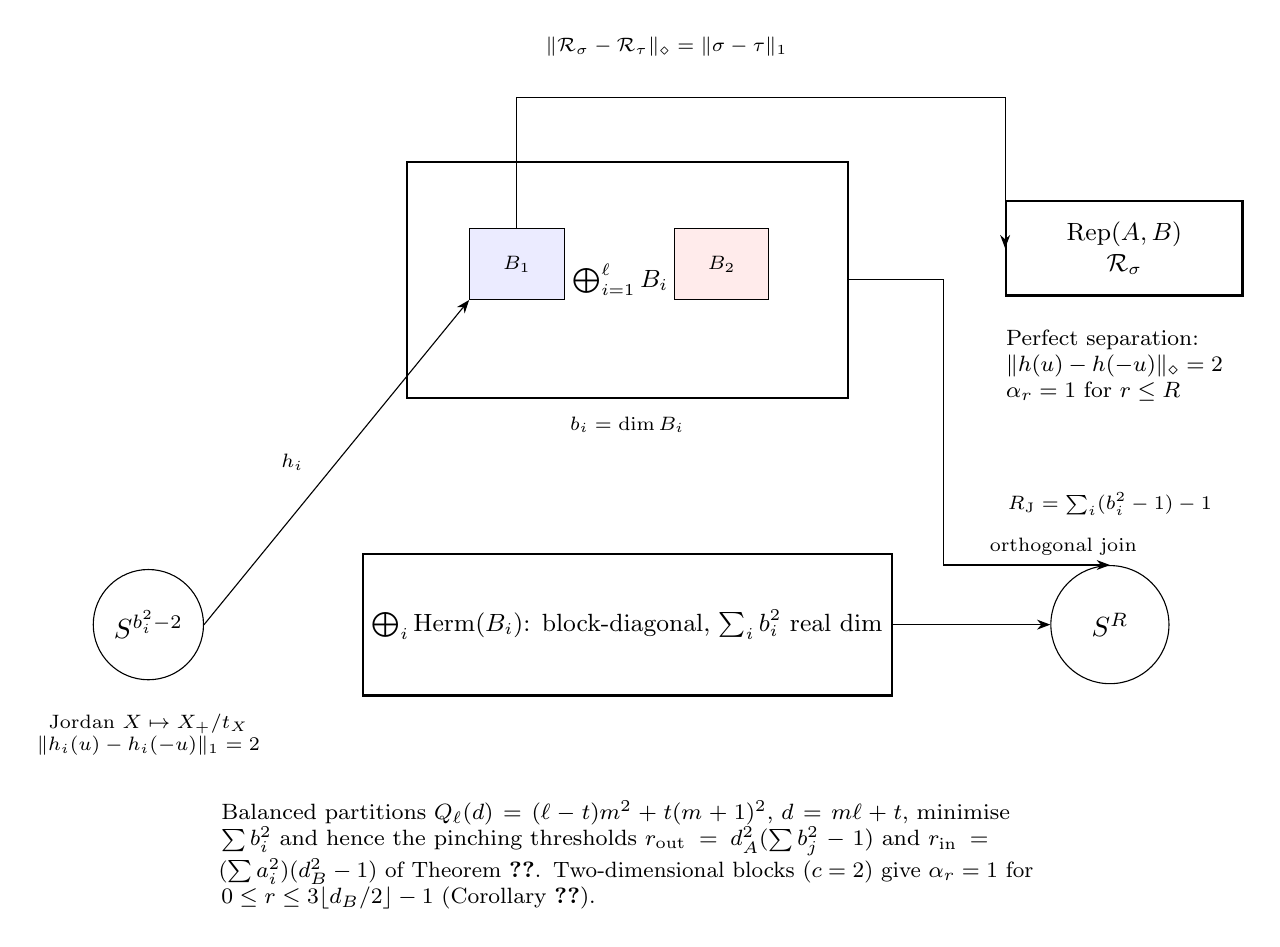
\begin{tikzpicture}[
  >=Stealth,
  block/.style={draw, thick, minimum width=18mm, minimum height=12mm, align=center, font=\small},
  smallblock/.style={draw, minimum width=12mm, minimum height=9mm, align=center, font=\scriptsize}
]

\node[block, minimum width=56mm, minimum height=30mm] (B) at (0,-10mm) {$B=\bigoplus_{i=1}^\ell B_i\oplus B_\perp$};
\node[smallblock, fill=blue!8] (B1) at (-14mm,-8mm) {$B_1$};
\node[smallblock, fill=red!8] (B2) at (12mm,-8mm) {$B_2$};
\node at (B.south) [below=1mm, font=\scriptsize] {$b_i=\dim B_i$};


\node[block, minimum width=56mm, minimum height=18mm] (FB) at (0,-53.8mm) {$\bigoplus_i\Herm(B_i)$: block-diagonal, $\sum_i b_i^2$ real dim};


\node[draw, circle, minimum size=14mm, left=20mm of FB] (S) {$S^{b_i^2-2}$};
\draw[->] (S.east) -- (B1.south west) node[midway, left, xshift=-3mm, font=\scriptsize] {$h_i$};
\node[below=3mm of S, font=\scriptsize, align=center] {Jordan $X\mapsto X_+/t_X$\\$\|h_i(u)-h_i(-u)\|_1=2$};


\node[draw, circle, minimum size=15mm, right=20mm of FB] (J) {$S^{R}$};
\node[above=5mm of J, font=\scriptsize, align=center] (Rlab) {$R_{\mathrm J}=\sum_i(b_i^2-1)-1$};

\draw[->] (B.east) -- ++(12mm,0) |- (J.north) node[pos=0.86, above, font=\scriptsize] {orthogonal join};
\draw[->] (FB.east) -- (J.west);


\node[block, right=10mm of B, minimum width=30mm, minimum height=12mm] (Rep) at (38mm,-6mm) {$\operatorname{Rep}(A,B)$\\$\mathcal R_{\sigma}$};

\coordinate (aboveB) at ($(B.north)+(0,8mm)$);
\draw[->] (B1.north) -- (B1.north |- aboveB) -- node[midway, above, yshift=4mm, xshift=-12mm, font=\scriptsize] {$\|\mathcal R_\sigma-\mathcal R_\tau\|_\diamond=\|\sigma-\tau\|_1$} (Rep.west |- aboveB) -- (Rep.west);


\node[below=3mm of Rep, font=\footnotesize, align=left, text width=30mm, anchor=north] (perf) {Perfect separation:\\$\|h(u)-h(-u)\|_\diamond=2$\\$\alpha_r=1$ for $r\le R$};


\node[below=12mm of FB, text width=0.85\linewidth, font=\footnotesize, align=left] (bal) {Balanced partitions $Q_\ell(d)=(\ell-t)m^2+t(m+1)^2$, $d=m\ell+t$, minimise $\sum b_i^2$ and hence the pinching thresholds $r_{\mathrm{out}}=d_A^2(\sum b_j^2-1)$ and $r_{\mathrm{in}}=(\sum a_i^2)(d_B^2-1)$ of Theorem~\ref{thm:block-pinching-upper}. Two-dimensional blocks ($c=2$) give $\alpha_r=1$ for $0\le r\le3\lfloor d_B/2\rfloor-1$ (Corollary~\ref{cor:block-envelope}).};
\end{tikzpicture}
\caption{Replacement-family geometry and orthogonal-block join. Each block $B_i$ carries a sphere $S^{b_i^2-2}$ with antipodal trace norm $2$ via the Jordan construction $X\mapsto X_+/{\rm Tr}X_+$ of Theorem~\ref{thm:full-state-antipodal}, restricted to $\Herm_0(B_i)$. Orthogonal supports make the trace norm additive, giving $\|H(y)-H(-y)\|_1=\sum_i\lambda_i\|h_i(u_i)-h_i(-u_i)\|_1$, which equals $2$ when every block sphere is perfectly separated (Proposition~\ref{prop:join}). The replacement isometry (Lemma~\ref{lem:replacement}) transfers this to diamond distance $2$ for channels; the $n$-outcome analogue for quantum instruments is developed in Ref.~\cite{CompanionInstruments}. Balanced $Q_\ell(d)$ minimise the pinching thresholds (Corollary~\ref{cor:balanced-pinching-upper}).}
\label{fig:replacement-join}
\end{figure}

Figure~\ref{fig:replacement-join} summarises the orthogonal-block join construction and the replacement isometry.

\subsection{Unitary Clifford sections}

Clifford sections additionally provide a unitary-channel family, whereas the
block-join construction of Figure~\ref{fig:replacement-join} (stated in
Appendix~\ref{app:partition-sections}) consists of replacement channels. Let
\[
\UChan(H)=\{\mathcal U_U:X\mapsto UXU^\dagger:U\in\mathrm U(H)\}.
\]

\begin{proposition}[Clifford replacement sections]
\label{prop:clifford-replacement}
Let $q=\lfloor\log_2d_B\rfloor$, $p=2^q$, and choose a
$p$-dimensional subspace $C\subseteq B$. There is a continuous family of
replacement channels on $S^{2q}$ with antipodal diamond distance $2$.
\end{proposition}

\begin{theorem}[Clifford unitary sections]
\label{thm:clifford-unitary}
If $A=B=H$ is square of dimension $d\geq2$, let $p=2^{\lfloor\log_2d\rfloor}$,
choose a $p$-dimensional subspace $C\subseteq H$, and let $H_u$ denote the
anticommuting generators on $C$ of Proposition~\ref{prop:clifford-replacement}.
The unitaries $U_u=(I_C+iH_u)/\sqrt2\oplus I_{C^\perp}$ give a family in
$\UChan(H)$ with the same antipodal distance.
\end{theorem}

The proofs are given in Appendix~\ref{app:clifford-proof}.


\begin{corollary}[Unitary-promise obstruction]
\label{cor:unitary-promise}
If $H\simeq\mathbb C^d$ and $q=\lfloor\log_2d\rfloor$, then
\[
\alpha_r(\UChan(H))=1,
\qquad0\leq r\leq2q.
\]
Consequently, every continuous encoder of the unitary promise class through
an $m$-dimensional quantum-state alphabet with $m^2-1\leq2q$ has worst-case
diamond reconstruction error at least $1$, even with an unrestricted
decoder.
\end{corollary}

\begin{proof}
Restrict the unitary Clifford sphere in Theorem~\ref{thm:clifford-unitary} to a
coordinate equator $S^r$. Its antipodes have diamond distance $2$, giving
the profile lower bound $1$; the universal channel-diameter bound gives the
reverse inequality. The state-space code embeds into
$\mathbb R^{m^2-1}$, so Proposition~\ref{prop:euclidean-coindex} and
Theorem~\ref{thm:intrinsic-latent} give the memory statement.
\end{proof}

\begin{proposition}[Unitary-promise zero-error coordinate bound]
\label{prop:unitary-coordinate-bound}
Let $H$ have dimension $d>1$. If a continuous encoder
$f:\UChan(H)\to\mathbb R^r$ admits an exact decoder on its image, then
\[
r\geq d^2.
\]
This is a lower bound on the Euclidean embedding dimension of the unitary promise class; whether $d^2$ coordinates admit an exact continuous encoder is not addressed here. At $d=2$ the bound is not sharp: $\UChan(\mathbb C^2)\simeq\mathrm{PU}(2)\cong\mathbb{RP}^3$ embeds in $\mathbb R^5$ but not in $\mathbb R^4$ (its minimal embedding dimension is $5$), so in fact $r\geq5$ there; the sharp embedding dimension of $\mathrm{PU}(d)$ for general $d$ is not pursued here.
\end{proposition}

\begin{proof}
Exact reconstruction forces $f$ to be injective. The unitary-channel space
is the compact boundaryless manifold
$\UChan(H)\simeq\mathrm{PU}(d)$ of real dimension $d^2-1$. The invariance
of dimension theorem excludes a topological embedding of this manifold into
$\mathbb R^r$ for $r<d^2-1$. If $r=d^2-1$, invariance of domain makes the
image of every coordinate
neighbourhood open in $\mathbb R^{d^2-1}$, so the image of the whole manifold
is open. It is also compact and nonempty, which is impossible in Euclidean
space. These standard invariance-of-dimension and invariance-of-domain
results are reviewed, for example, in~\cite{Munkres2000}.
\end{proof}

\begin{corollary}[Exact width of the Clifford replacement sphere]
\label{cor:clifford-exact}
Let $\mathcal K_{\mathrm{Cl}}=
\{\mathcal R_{\sigma_u}:u\in S^{2q}\}$, where the Clifford generators $H_u$,
the projector $P_C$, and the states $\sigma_u=(P_C+H_u)/p$ are as in
Appendix~\ref{app:clifford-proof}. Then
\[
\delta_r^{\mathrm c}(\mathcal K_{\mathrm{Cl}};\Chan(A,B))=1,
\qquad0\leq r\leq2q.
\]
\end{corollary}

\begin{proof}
The defining sphere has antipodal distance $2$, so its profile is $1$ on
the stated range and Theorem~\ref{thm:profile-fiber} gives the lower bound.
For the upper bound, use the constant decoder $\mathcal R_{P_C/p}$; the
operator $P_C/p$ is a state on $B$ supported on $C$ because $\Tr P_C=p$. Since
$\|H_u\|_1=p$ (eigenvalues $\pm1$ equal multiplicity),
\[
\|\mathcal R_{\sigma_u}-\mathcal R_{P_C/p}\|_\diamond=1.
\]
\end{proof}

\subsection{Observable and full-direction sections}

\begin{theorem}[Observable antipodal sphere]
\label{thm:observable-channel}
Assume $d_A\ge2$ and $d_B\ge2$. Then there exists a continuous map
$h:S^{d_A^2-2}\to\Chan(A,B)$ whose antipodal images have diamond distance
$2$; consequently
\[
\alpha_r(\Chan(A,B))=1\qquad(0\le r\le d_A^2-2).
\]
This is the $n=1$ case of the observable-sphere theorem for $n$-outcome
quantum instruments proved in Ref.~\cite{CompanionInstruments}.
\end{theorem}

\begin{proof}
Fix two orthogonal pure states $\sigma_+,\sigma_-$ on $B$. For
$H\in\Herm_0(A)$, $H\neq0$, set $K(H)=H/\|H\|_\infty$ and
$E_\pm(H)=(I_A\pm K(H))/2$. Then $E_\pm(H)\ge0$ and
$E_+(H)+E_-(H)=I_A$, so
\[
\Phi^H(X)=\Tr(E_+(H)X)\,\sigma_++\Tr(E_-(H)X)\,\sigma_-
\]
is a channel. The Hermitian operator $K(H)$ has norm one, so it admits a unit
eigenvector $|\psi\rangle$ with eigenvalue $\varepsilon\in\{+1,-1\}$; for
that vector one effect has expectation one and the other expectation
zero. Since
$E_\pm(-H)=E_\mp(H)$, the outputs of $\Phi^H$ and $\Phi^{-H}$ on the input
$|\psi\rangle\langle\psi|$ are $\sigma_\varepsilon$ and
$\sigma_{-\varepsilon}$, which are orthogonal, so their trace norm is
$2$; the diamond distance is therefore exactly $2$ by the diameter bound.
Normalisation $H\mapsto H/\|H\|_\infty$ is continuous away from zero,
hence on the compact unit sphere of $\Herm_0(A)\cong\mathbb R^{d_A^2-1}$;
the antipodal images thus form a continuous sphere with diamond distance
$2$, and coordinate equators supply every smaller index.
\end{proof}

\begin{theorem}[Full-direction antipodal sphere]
\label{thm:full-direction-channel}
Assume $d_B>1$, and let $D=D_{A,B}$. For every $0\le r\le D-1$ there
exists a continuous map $h:S^r\to\Chan(A,B)$ such that
\[
\|h(u)-h(-u)\|_\diamond\ge\frac2{d_A}
\qquad\forall u\in S^r.
\]
Consequently $\alpha_r(\Chan(A,B))\ge1/d_A$ for all $0\le r<D$. If
$d_A=1$ the separation equals $2$, so $\alpha_r=1$ for all $r<D_{1,B}$,
matching the exact replacement profile. This is the $n=1$ case of
the corresponding instrument theorem in Ref.~\cite{CompanionInstruments}.
\end{theorem}

\begin{proof}
This is the $n=1$ specialisation of the full-direction theorem for instruments proved in Ref.~\cite{CompanionInstruments}, obtained by deleting the flag register; the channel-level construction and its complete verification are as follows. Let $\mathcal V=\{Z\in\Herm(A_0\otimes B):\Tr_BZ=0\}$ be the direction space, of real dimension $D$, equipped with a Euclidean norm and unit sphere $S(\mathcal V)\cong S^{D-1}$. For $Z\in S(\mathcal V)$ write the Jordan decomposition $Z=Z_+-Z_-$; since $\Tr_BZ=0$, the partial traces of $Z_+$ and $Z_-$ agree, and $t:=\Tr Z_+=\Tr Z_-$ is positive: $t=0$ would give $Z=-Z_-\le0$, and $\Tr Z=0$ then forces $Z=0$. Set $\Theta_\pm=Z_\pm/t$ and $\mu=\Tr_B\Theta_+=\Tr_B\Theta_-$; the states $\Theta_+$ and $\Theta_-$ have orthogonal supports and common $A_0$-marginal $\mu$. If $d_A=1$ set $J^\pm(Z)=\Theta_\pm$. If $d_A\ge2$, set $\lambda=1/d_A$, $\nu=(I_{A_0}-\mu)/(d_A-1)\ge0$, and $J^\pm(Z)=\lambda\Theta_\pm+(1-\lambda)\nu\otimes(I_B/d_B)$. In both cases $J^\pm(Z)\ge0$ and $\Tr_BJ^\pm(Z)=\lambda\mu+(1-\lambda)\nu=I_{A_0}/d_A$, so $J^\pm(Z)$ are normalised Choi operators of channels; let $h(Z)$ be the channel with Choi operator $J^+(Z)$. The remaining verification is as follows: $h(-Z)$ has Choi operator $J^-(Z)$; the antipodal Choi difference $J^+(Z)-J^-(Z)=\lambda(\Theta_+-\Theta_-)$ has trace norm $2\lambda=2/d_A$, which by \eqref{eq:choi-diamond} gives the claimed diamond separation; and $Z\mapsto J^+(Z)$ is continuous because $Z\mapsto Z_+$ is continuous and $t$ is bounded away from zero on the compact sphere. Restricting to coordinate equators covers all smaller dimensions $r$.
\end{proof}

\begin{proposition}[Observable--replacement join]
\label{prop:join-channel}
Assume $d_A\ge2$ and $d_B\ge3$. Then
\[
\alpha_r(\Chan(A,B))=1
\qquad(0\le r\le d_A^2+(d_B-2)^2-3).
\]
This is the $n=1$ case of the instrument-level join of
Ref.~\cite{CompanionInstruments}: at $n=1$ the join threshold
$N_{\mathrm{join}}=(d_B-2)^2\ge1$ is equivalent to $d_B\ge3$, the boundary
value $N_{\mathrm{join}}=1$ (i.e.\ $d_B=3$) being the degenerate case in which
the replacement component is the empty sphere and the observable component
alone realises the full range.
\end{proposition}

\begin{proof}
Let $W_2=\operatorname{span}\{|\varphi_+\rangle,|\varphi_-\rangle\}$
be the two-dimensional subspace spanned by the orthogonal output states of
the observable sphere in Theorem~\ref{thm:observable-channel}; every
channel in that sphere has output supported on $W_2$. Let $W_2^\perp$ be
its orthogonal complement, of dimension $d_B-2\ge1$. If $d_B=3$, then
$(d_B-2)^2-2=-1$: the space $\Herm_0(W_2^\perp)$ is trivial, the replacement
sphere $S^{(d_B-2)^2-2}$ is empty, and the claimed range
$d_A^2+(d_B-2)^2-3=d_A^2-2$ is that of the observable sphere alone
(Theorem~\ref{thm:observable-channel}, applicable since $d_B\ge2$); assume
henceforth $d_B\ge4$, so that $(d_B-2)^2-2\ge2$ and the replacement sphere
is nonempty. The Jordan
construction of Theorem~\ref{thm:full-state-antipodal}, restricted to
$\Herm_0(W_2^\perp)\subseteq\Herm_0(B)$, gives a continuous map
$h_{\mathrm{rep}}:S^{(d_B-2)^2-2}\to\Sstate(W_2^\perp)$ whose antipodes have
orthogonal supports; by Lemma~\ref{lem:replacement} the corresponding
replacement channels have antipodal diamond distance $2$. For
$y=(y_1,y_2)$ on the join sphere
$S^{(d_A^2-2)+((d_B-2)^2-2)+1}$ with $\lambda=\|y_1\|_2^2$, set
$u_1=y_1/\|y_1\|_2$ and $u_2=y_2/\|y_2\|_2$ where the corresponding blocks
are nonzero, and define
\[
H(y)(X)=\lambda\,\Phi^{u_1}(X)+(1-\lambda)\,\mathcal R_{\tau_{u_2}}(X),
\]
setting the corresponding term to zero when its block vanishes. The
endpoint cases $\lambda\in\{0,1\}$ reduce to a single component, at distance
$2$, so assume $0<\lambda<1$. Both
summands are channels, so $H(y)$ is a channel; continuity at vanishing
blocks holds as in Proposition~\ref{prop:join}, since each vanishing term
is bounded in diamond norm by the vanishing weight. On the input
$|\psi\rangle\langle\psi|$ exposing the pair $(\Phi^{u_1},\Phi^{-u_1})$,
the output of $H(y)-H(-y)$ splits into the part
$\lambda(\sigma_\varepsilon-\sigma_{-\varepsilon})$ supported on $W_2$ and
the part $(1-\lambda)(\tau_{u_2}-\tau_{-u_2})$ supported on $W_2^\perp$; the two supports are mutually orthogonal and each part has
trace norm $2\lambda$, respectively $2(1-\lambda)$, so the total trace
norm is $2$, and the diamond distance is exactly $2$ by the diameter bound.
Restriction to coordinate equators supplies every smaller index, and
$\alpha_r\le1$ always by the diameter bound.
\end{proof}

\begin{theorem}[Global in-radius and the optimal centred ball]
\label{thm:global-inradius-channel}
For every $\Phi_0\in\Chan(A,B)$,
\[
\rho_\diamond(\Phi_0)\le\rho_\diamond(\Omega_{A,B})=\rhodep(A,B).
\]
Thus $\rhodep(A,B)$ is the largest relative ball contained in the channel
body about any centre, and the centred-ball term of the certified envelope
cannot be improved by re-centring. The concavity argument is the $n=1$
case of the instrument-level statement of Ref.~\cite{CompanionInstruments}.
\end{theorem}

\begin{proof}
For a convex body $K$ in a finite-dimensional normed affine space, the
relative in-radius about any centre $x\in K$ equals the infimum over closed
halfspaces $H\supseteq K$ of the distance from $x$ to $\partial H$: the ball
$B(x,\rho)\subseteq K$ holds if and only if $B(x,\rho)\subseteq H$ for every
such $H$, by separation, and the two infima coincide (at a
relative-boundary centre a supporting halfspace contains the centre on its
boundary, and both sides vanish). Each map
$x\mapsto\operatorname{dist}(x,\partial H)$ is affine, so the in-radius is
a pointwise infimum of affine functions, hence concave on $K$. The in-radius
is moreover $1$-Lipschitz, hence continuous: $B(x,\rho)\subseteq K$ implies
$B(x',\rho-\|x'-x\|)\subseteq K$ by the triangle inequality, so
$\rho_\diamond(\Phi_0')\ge\rho_\diamond(\Phi_0)-\|\Phi_0'-\Phi_0\|_\diamond$,
and symmetrically.

For $V\in\mathrm U(B)$ let $T_V(\Psi)=\mathcal C_V\circ\Psi$ with
$\mathcal C_V(Y)=VYV^\dagger$. This is an affine isometry of
$\Chan(A,B)$ by unitary invariance of the diamond norm, so
$\rho_\diamond(T_V(\Phi_0))=\rho_\diamond(\Phi_0)$. The Haar barycentre of
$\Phi_0$ under this action is $\Omega_{A,B}$: averaging first over
$\mathrm U(B)$, Schur's lemma gives
$\int V\Psi(X)V^\dagger\,dV=(\Tr\Psi(X)/d_B)I_B$, and $\Tr\Psi(X)=\Tr X$
for the trace-preserving $\Psi$, so the barycentre maps
$X\mapsto\Tr(X)I_B/d_B=\Omega_{A,B}(X)$. Jensen's inequality for the concave
continuous in-radius (applied to finite convex combinations of orbit points
and extended to the Haar integral by continuity) gives
\[
\rho_\diamond(\Omega_{A,B})
=\rho_\diamond\Big(\int T_V(\Phi_0)\,dV\Big)
\ge\int\rho_\diamond(T_V(\Phi_0))\,dV
=\rho_\diamond(\Phi_0),
\]
as claimed.
\end{proof}

\subsection{The channel lower envelope}

The replacement, observable, and joined spheres supply the strongest bound
at small indices, while the globally optimal centred ball and the
full-direction section remain available throughout the full affine range.
The following envelope records their pointwise maxima and keeps its positive
entries separate from the exact zero-error threshold.

\begin{definition}[Certified channel lower envelope]
\label{def:channel-envelope}
Set
\[
L_{\mathrm{rep}}=d_B^2-2,
\]
\[
L_{\mathrm{obs}}=
\begin{cases}
d_A^2-2,&d_A\ge2,\ d_B\ge2,\\
-1,&\text{otherwise},
\end{cases}
\qquad
L_{\mathrm{join}}=
\begin{cases}
d_A^2+(d_B-2)^2-3,&d_A\ge2,\ d_B\ge3,\\
-1,&\text{otherwise},
\end{cases}
\]
and
\[
L_{A,B}
=\min\Big\{D_{A,B}-1,\ \max\{L_{\mathrm{rep}},L_{\mathrm{obs}},L_{\mathrm{join}}\}\Big\},
\qquad
\gamma_{A,B}
=\max\Big\{\rhodep(A,B),\ \frac1{d_A}\Big\}.
\]
Then
\[
\beta_r(A,B)=
\begin{cases}
2-\rhodep(A,B),&r=0,\\[2pt]
1,&1\le r\le L_{A,B},\\[2pt]
\gamma_{A,B},&L_{A,B}<r<D_{A,B},\\[2pt]
0,&r\ge D_{A,B}.
\end{cases}
\]
When $d_A=1$ the observable and join terms are vacuous and
$L_{1,B}=d_B^2-2=D_{1,B}-1$, so the middle range is empty. The value at
$r=0$ is the exact constant-code width
(Theorems~\ref{thm:depolarizing-chebyshev} and~\ref{thm:exact-chebyshev-radius}):
the envelope is upgraded there from the one-sphere value $1$ to
$2-\rhodep(A,B)$, so the lower and upper envelopes coincide at $r=0$.
Since $d_B\min\{d_A,d_B\}\ge2$ gives $2-\rhodep(A,B)\ge1$ and $d_A\ge1$ gives
$0<\gamma_{A,B}\le1$, the displayed envelope is non-increasing. Each component is certified by
Theorems~\ref{thm:full-state-antipodal}, \ref{thm:observable-channel}, and
\ref{thm:full-direction-channel}, Proposition~\ref{prop:join-channel}, and
Theorem~\ref{thm:bottleneck}; the ball term $\rhodep(A,B)$ is the exact
centred radius of Theorem~\ref{thm:exact-inradius}, whose optimality among
all centres is Theorem~\ref{thm:global-inradius-channel}; the value at
$r=0$ is the exact constant-code width of
Theorems~\ref{thm:depolarizing-chebyshev} and~\ref{thm:exact-chebyshev-radius}. The
quantity $L_{A,B}$ is the $n=1$ value of the separation index and
$\gamma_{A,B}$ the $n=1$ envelope value of the instrument-level theory
of Ref.~\cite{CompanionInstruments}.
\end{definition}

\begin{remark}[Certified envelope]
The envelope $\beta_r$ is a certified lower bound, exact at $r=0$.
The drop from $1$ to $\gamma_{A,B}$ at $r=L_{A,B}$ records the certified constructions used here (replacement, observable, and joined spheres; the globally optimal centred ball of Theorem~\ref{thm:global-inradius-channel}; the full-direction section), not an exact evaluation of $\alpha_r(\Chan(A,B))$, which may remain larger than $\gamma_{A,B}$ for some $r>L_{A,B}$.
\end{remark}

\begin{theorem}[Channel reconstruction lower envelope]
\label{thm:hierarchy}
Let $\TPHP(A,B)$ be the affine space of Hermiticity-preserving,
trace-preserving maps with diamond distance, and define
\begin{align*}
\widetilde\delta_r^\diamond(A,B)
&=\delta_r^{\mathrm c}(\Chan(A,B);\TPHP(A,B)),\\
\delta_r^\diamond(A,B)
&=\delta_r^{\mathrm c}(\Chan(A,B);\Chan(A,B)).
\end{align*}
Then
\[
\delta_r^\diamond(A,B)
\geq\widetilde\delta_r^\diamond(A,B)
\geq\alpha_r(\Chan(A,B))
\geq\beta_r(A,B).
\]
Moreover,
\[
\widetilde\delta_r^\diamond(A,B)=\delta_r^\diamond(A,B)=0
\qquad(r\geq D_{A,B}).
\]
The positive values in $\beta_r$ are lower bounds; the zero-error threshold
is exact. Note that $\widetilde\delta_r^\diamond\le\delta_r^\diamond$, so vanishing of $\delta_r^\diamond$ implies vanishing of $\widetilde\delta_r^\diamond$.
\end{theorem}

\begin{proof}
Every channel-valued decoder is $\TPHP(A,B)$-valued, which gives the first
inequality. Theorem~\ref{thm:profile-fiber} gives the second. At $r=0$ every encoder is constant, and
Theorem~\ref{thm:depolarizing-chebyshev} gives
$\delta_0^\diamond(A,B)=\widetilde\delta_0^\diamond(A,B)=2-\rhodep(A,B)=\beta_0(A,B)$,
so the bracket is exact at $r=0$.
Theorem~\ref{thm:full-state-antipodal}, Theorem~\ref{thm:observable-channel}, and
Proposition~\ref{prop:join-channel} give the value one through index
$L_{A,B}$. For $L_{A,B}<r<D_{A,B}$, the radial map of
Theorem~\ref{thm:bottleneck}, applied to the exact centred ball of
Theorem~\ref{thm:exact-inradius} (optimal among all centres by
Theorem~\ref{thm:global-inradius-channel}, so re-centring cannot certify
more), gives the lower bound $\rhodep(A,B)$, and Theorem~\ref{thm:full-direction-channel} gives the
lower bound $1/d_A$; the pointwise maximum is $\gamma_{A,B}$.
Proposition~\ref{prop:euclidean-threshold} gives
exact reconstruction at and above $D_{A,B}$.
\end{proof}

\begin{remark}[Output preparation and dynamical response]
The breakpoint $L_{A,B}+1$ separates two scales, an input-independent one
and an input-dependent one. A single
output density operator carries $d_B^2-1$ affine parameters, while an
input-dependent channel carries $d_A^2(d_B^2-1)$. Up to $L_{A,B}$, error one is forced by two effects: preparing and
recording an output state alone obstructs the range up to $d_B^2-2$, and
input-dependent effect readout --- the observable sphere
(Theorem~\ref{thm:observable-channel}) and its join with the replacement
sphere (Proposition~\ref{prop:join-channel}) --- extends the obstruction
whenever $d_A^2\ge4d_B-2$, in particular for every square system of
dimension at least four. Beyond $L_{A,B}$, what remains to be resolved is
the dependence of the output on the input operator; there the globally
optimal centred ball and the full-direction section certify
$\gamma_{A,B}=\max\{\rhodep(A,B),1/d_A\}$, and for $d_A\le d_B$ the
input-dependent term dominates, so $\gamma_{A,B}=1/d_A$. The two scales
distinguish output-state complexity from input-dependent process response;
they do not imply a decomposition theorem for optimal physical encoders.
\end{remark}

\begin{definition}[Perfect-separation indices]
Define
\[
\pi(A,B)=\sup\{r\in\mathbb N_0:\alpha_r(\Chan(A,B))=1\},
\]
and
\[
\pi_{\mathrm U}(d)
=\sup\{r\in\mathbb N_0:
\alpha_r(\UChan(\mathbb C^d))=1\}.
\]
\end{definition}

\begin{corollary}[Known perfect-separation ranges]
\label{cor:perfect-separation-indices}
The proved bounds are
\[
L_{A,B}\leq\pi(A,B)\leq D_{A,B}-1,
\]
and, for every $d\geq2$,
\[
2\lfloor\log_2d\rfloor
\leq\pi_{\mathrm U}(d)
\leq2d^2-3.
\]
The replacement-family index is exactly $d_B^2-2$ by
Proposition~\ref{prop:replacement-perfect-index}. When $d_A=1$, the channel
body is the output state space, and therefore
\[
\pi(A,B)=d_B^2-2.
\]
\end{corollary}

\begin{proof}
The lower bound on $\pi(A,B)$ follows from Theorems~\ref{thm:full-state-antipodal} and~\ref{thm:observable-channel} and from Proposition~\ref{prop:join-channel}; the unitary bounds follow from Corollary~\ref{cor:unitary-promise}. For $r\geq D_{A,B}$, affine
coordinates and Borsuk--Ulam force an antipodal collision for every map from
$S^r$ into the channel body. Hence $\alpha_r=0$ throughout that range.

The manifold $\UChan(\mathbb C^d)\simeq\mathrm{PU}(d)$ has real dimension
$d^2-1$. Whitney's embedding theorem gives an embedding into
$\mathbb R^{2d^2-2}$~\cite{Hirsch1976}. Proposition
\ref{prop:euclidean-coindex} then gives
$\alpha_r(\UChan(\mathbb C^d))=0$ for $r\geq2d^2-2$, proving the unitary
upper bound.
\end{proof}

\subsection{Constant reconstruction and Chebyshev geometry}

The lower envelope does not determine the positive full-channel widths. A
complementary upper bound is obtained from constant reconstruction. For
$r=0$, this is the entire coding problem, so its minimax radius can be
evaluated exactly before being used at every larger latent dimension.

\begin{theorem}[Depolarizing channel as a Chebyshev centre]
\label{thm:depolarizing-chebyshev}
For $\Psi\in\TPHP(A,B)$ define
\[
R(\Psi)=\sup_{\Phi\in\Chan(A,B)}\|\Phi-\Psi\|_\diamond.
\]
Then
\[
R(\Omega_{A,B})\leq R(\Psi)
\qquad\text{for every }\Psi\in\TPHP(A,B).
\]
Consequently,
\[
\widetilde\delta_0^\diamond(A,B)
=\delta_0^\diamond(A,B)
=\sup_{\Phi\in\Chan(A,B)}
\|\Phi-\Omega_{A,B}\|_\diamond.
\]
Uniqueness of the optimal centre is left open.
\end{theorem}

\begin{proof}
For $V\in\mathrm U(B)$, let
$\mathcal C_V(Y)=VYV^\dagger$ and
$T_V(\Psi)=\mathcal C_V\circ\Psi$. This is an affine bijection of both
$\Chan(A,B)$ and $\TPHP(A,B)$, and unitary invariance of the diamond norm
gives $R(T_V(\Psi))=R(\Psi)$. The function $R$ is convex because it is a
supremum of norm-distance functions.

Let $dV$ be normalised Haar measure and put
$\mathcal T(Y)=\int VYV^\dagger\,dV$. Haar invariance implies
$W\mathcal T(Y)W^\dagger=\mathcal T(Y)$ for every unitary $W$ on $B$.
Thus $\mathcal T(Y)$ is scalar, and trace preservation of the integral fixes
the scalar:
\[
\mathcal T(Y)=\frac{\Tr Y}{d_B}I_B.
\]
Therefore every trace-preserving $\Psi$ satisfies
\[
\int_{\mathrm U(B)}T_V(\Psi)(X)\,dV
=\frac{\Tr\Psi(X)}{d_B}I_B
=\Omega_{A,B}(X).
\]
Jensen's inequality now gives
\[
R(\Omega_{A,B})
\leq\int R(T_V(\Psi))\,dV
=R(\Psi).
\]
Taking the infimum over $\TPHP(A,B)$ and over its subset $\Chan(A,B)$
proves the two equalities.
\end{proof}

\begin{theorem}[Exact Chebyshev covering radius]
\label{thm:exact-chebyshev-radius}
Let $s=\min\{d_A,d_B\}$. Then
\[
R(\Omega_{A,B})
=2\left(1-\frac1{d_Bs}\right)
=2-\rhodep(A,B).
\]
Consequently,
\[
\widetilde\delta_0^\diamond(A,B)
=\delta_0^\diamond(A,B)
=2-\rhodep(A,B).
\]
\end{theorem}

The proof is given in Appendix~\ref{app:chebyshev-radius-proof}.

\begin{remark}[Local robustness and maximal departure from noise]
The exact formulas give the special identity
\[
\rho_\diamond(\Omega_{A,B})+R(\Omega_{A,B})=2.
\]
This is not a generic in-radius/covering-radius relation for convex bodies.
Here the same effective support size
$d_B\min\{d_A,d_B\}$ controls both the nearest loss of complete positivity
under a trace-preserving perturbation and the largest entanglement-assisted
diamond distance from complete depolarization. The identity therefore links
a local robustness property of the noisy centre to a global discrimination
extremum of the channel body.
\end{remark}

\begin{proposition}[Fixed-marginal Chebyshev centre]
\label{prop:fixed-marginal-chebyshev}
Let $K\subseteq\Chan(A,B_1\otimes B_2)$ be compact and invariant under
post-composition by the conjugation channel
$\operatorname{id}_{B_1}\otimes\mathcal C_V$, where
$\mathcal C_V(Y)=VYV^\dagger$ and $V\in\mathrm U(B_2)$. Suppose
\[
\Tr_{B_2}\circ\Phi=\Lambda
\qquad(\Phi\in K)
\]
for one fixed channel $\Lambda:A\to B_1$. Among Hermiticity-preserving,
trace-preserving centres with this marginal, the channel
\[
\Phi_0(X)=\Lambda(X)\otimes\frac{I_{B_2}}{d_{B_2}}
\]
minimises the worst-case diamond distance to $K$.
\end{proposition}

The proof is given in Appendix~\ref{app:fixed-marginal-proof}.

\subsection{Constructive intermediate-dimensional upper bounds}

The constant decoder gives an upper bound at every latent dimension but does
not use the available coordinates. Two additional constructions provide
nontrivial upper bounds: affine projection controls fibers near the full
affine threshold, while physical pinching retains selected coherent input or
output sectors. Figure~\ref{fig:replacement-join} illustrates the orthogonal-block join and how balanced partitions $Q_\ell(d)$ minimize the pinching thresholds $r_{\rm out},r_{\rm in}$; Figure~\ref{fig:qubit-envelope} shows the resulting upper envelope $U_r$ versus the lower envelope $\beta_r$ for qubits.

\begin{lemma}[Exact diamond norm of a pinching error]
\label{lem:pinching-diamond}
Let $H=\bigoplus_{j=1}^{\ell}H_j$ be an orthogonal decomposition into
nonzero subspaces, with projections $P_j$, and define
\[
\mathcal P_H(X)=\sum_{j=1}^{\ell}P_jXP_j.
\]
Then
\[
\|\operatorname{id}_H-\mathcal P_H\|_\diamond
=2\left(1-\frac1\ell\right).
\]
\end{lemma}

\begin{proof}
Let $\omega=e^{2\pi i/\ell}$ and set
\[
U_m=\sum_{j=1}^{\ell}\omega^{m(j-1)}P_j,
\qquad 0\leq m<\ell.
\]
The roots-of-unity identity
\[
\frac1\ell\sum_{m=0}^{\ell-1}
\omega^{m(i-j)}=\delta_{ij}
\]
shows that averaging the conjugation channels gives
\[
\mathcal P_H=\frac1\ell\sum_{m=0}^{\ell-1}\mathcal U_{U_m}.
\]
Hence
\[
\|\operatorname{id}_H-\mathcal P_H\|_\diamond
\leq\frac1\ell\sum_{m=1}^{\ell-1}
\|\operatorname{id}_H-\mathcal U_{U_m}\|_\diamond
\leq2\left(1-\frac1\ell\right).
\]
For the reverse inequality, choose unit vectors $|e_j\rangle\in H_j$ and
put $|e\rangle=\ell^{-1/2}\sum_j|e_j\rangle$. On their span,
\[
(\operatorname{id}_H-\mathcal P_H)(|e\rangle\langle e|)
=\frac1\ell(J_\ell-I_\ell),
\]
where $J_\ell$ is the all-ones matrix. Its eigenvalues are
$(\ell-1)/\ell$ and $-1/\ell$ with multiplicity $\ell-1$, so its trace
norm is $2(1-1/\ell)$. Evaluation on this input gives the matching diamond
lower bound.
\end{proof}

\begin{theorem}[Input- and output-pinching achievability]
\label{thm:block-pinching-upper}
The following bounds hold.
\begin{enumerate}
\item Let $B=\bigoplus_{j=1}^{\ell}B_j$, with
$b_j=\dim B_j>0$, and put
\[
r_{\mathrm{out}}
=d_A^2\left(\sum_{j=1}^{\ell}b_j^2-1\right).
\]
Then, for $r\geq r_{\mathrm{out}}$,
\[
\widetilde\delta_r^\diamond(A,B)
\leq\delta_r^\diamond(A,B)
\leq2\left(1-\frac1\ell\right).
\]
\item Let $A=\bigoplus_{i=1}^{k}A_i$, with
$a_i=\dim A_i>0$, and put
\[
r_{\mathrm{in}}
=\left(\sum_{i=1}^{k}a_i^2\right)(d_B^2-1).
\]
Then, for $r\geq r_{\mathrm{in}}$,
\[
\widetilde\delta_r^\diamond(A,B)
\leq\delta_r^\diamond(A,B)
\leq2\left(1-\frac1k\right).
\]
\end{enumerate}
In both cases the decoder may be chosen channel-valued.
\end{theorem}

\begin{proof}
For output pinching, let $\mathcal P_B$ be the channel from
Lemma~\ref{lem:pinching-diamond} and set
\[
K_{\mathrm{out}}
=\{\Psi\in\Chan(A,B):\mathcal P_B\circ\Psi=\Psi\}.
\]
The normalised Choi operators of this family are block diagonal in the
output decomposition. Their ambient real vector space has dimension
$d_A^2\sum_jb_j^2$. The marginal map
\[
\bigoplus_j\Herm(A_0\otimes B_j)\longrightarrow\Herm(A_0),
\qquad
(X_j)_j\longmapsto\sum_j\Tr_{B_j}X_j,
\]
is surjective: for $H\in\Herm(A_0)$, set
$X_1=H\otimes I_{B_1}/b_1$ and all other blocks to zero. Hence trace
preservation imposes $d_A^2$ independent affine equations. The depolarizing
channel belongs to the family and has
positive-definite Choi operator. Thus
$\dim_{\mathrm{aff}}K_{\mathrm{out}}=r_{\mathrm{out}}$.

Choose affine coordinates on this family and encode
$\mathcal P_B\circ\Phi$. Invert the coordinates on the encoded image and
use any fixed channel, e.g., $\Omega_{A,B}$, elsewhere; since no decoder
regularity is required, this is admissible. This gives a continuous encoder and a
channel-valued decoder satisfying
\begin{align*}
\|\Phi-\mathcal P_B\circ\Phi\|_\diamond
&\leq
\|\operatorname{id}_B-\mathcal P_B\|_\diamond
\|\Phi\|_\diamond\\
&=2\left(1-\frac1\ell\right).
\end{align*}
Padding by zero coordinates handles every $r\geq r_{\mathrm{out}}$.

For input pinching, let $\mathcal P_A$ be the corresponding channel on
$A$. On the Choi reference, use the basis-conjugate decomposition
$A_0=\bigoplus_i\overline A_i$. The Choi operators of channels satisfying
$\Psi\circ\mathcal P_A=\Psi$ are block diagonal in these input blocks. The
ambient block space has dimension $d_B^2\sum_i a_i^2$. The blockwise
marginal map is surjective by placing
$H_i\otimes I_B/d_B$ in each prescribed input block, so the constraints have
total rank $\sum_i a_i^2$. The depolarizing
channel is again a positive-definite relative interior point, giving affine
dimension $r_{\mathrm{in}}$.

Encode $\Phi\circ\mathcal P_A$ by affine coordinates and invert on the
image, defining it as $\Omega_{A,B}$ outside the image. Submultiplicativity and Lemma~\ref{lem:pinching-diamond} give
\[
\|\Phi-\Phi\circ\mathcal P_A\|_\diamond
\leq\|\operatorname{id}_A-\mathcal P_A\|_\diamond
=2\left(1-\frac1k\right).
\]
This proves the second claim.
\end{proof}

\begin{lemma}[Balanced partitions minimise squared block sums]
\label{lem:balanced-channel}
For $1\leq\ell\leq d$, write $d=m\ell+t$, $0\leq t<\ell$. Among all
partitions of $d$ into $\ell$ positive parts, the sum of squared parts is
minimised by the balanced partition with $\ell-t$ parts equal to $m$ and
$t$ parts equal to $m+1$, and the minimum is
\[
Q_\ell(d)=(\ell-t)m^2+t(m+1)^2.
\]
\end{lemma}

\begin{proof}
If two block sizes satisfy $a\ge b+2$, moving one dimension from the
larger to the smaller changes their squared sum by $-2(a-b-1)<0$; each
exchange strictly decreases the sum and there are only finitely many
partitions of $d$ into $\ell$ positive parts, so iteration terminates at
the balanced partition.
\end{proof}

\begin{corollary}[Balanced pinching bounds]
\label{cor:balanced-pinching-upper}
For $1\leq\ell\leq d_B$,
\[
\delta_r^\diamond(A,B)
\leq2\left(1-\frac1\ell\right)
\quad\text{if}\quad
r\geq d_A^2\bigl(Q_\ell(d_B)-1\bigr).
\]
For $1\leq k\leq d_A$,
\[
\delta_r^\diamond(A,B)
\leq2\left(1-\frac1k\right)
\quad\text{if}\quad
r\geq Q_k(d_A)(d_B^2-1).
\]
The same bounds hold for $\widetilde\delta_r^\diamond(A,B)$.
\end{corollary}

\begin{proof}
Choose balanced block decompositions in
Theorem~\ref{thm:block-pinching-upper}. Lemma~\ref{lem:balanced-channel}
shows that they minimise the required affine dimension for a fixed number
of blocks.
\end{proof}

In particular, a balanced two-sector output pinching gives
\[
\delta_r^\diamond(A,B)\leq1
\quad\text{for}\quad
r\geq d_A^2\left(
\left\lfloor\frac{d_B}{2}\right\rfloor^2+
\left\lceil\frac{d_B}{2}\right\rceil^2-1
\right),
\]
while complete output pinching gives
\[
\delta_r^\diamond(A,B)
\leq2\left(1-\frac1{d_B}\right)
\quad\text{for}\quad
r\geq d_A^2(d_B-1).
\]

\begin{remark}[Operational meaning of pinching]
Output pinching is fixed CPTP postprocessing and preserves every observable
that is block diagonal in the selected output sectors. Input pinching is
fixed CPTP preprocessing and preserves the channel action on every
block-diagonal input state. The diamond bounds quantify the worst loss of
inter-sector coherence under arbitrary entangled probes and output
measurements. The subsequent affine-coordinate decoder remains the
unrestricted representational decoder, not a fixed programmable processor.
\end{remark}

\begin{definition}[Constructive channel upper envelope]
\label{def:channel-upper-envelope}
For $0\leq r\leq D_{A,B}$, let $U_r(A,B)$ be the minimum of
\[
2-\rhodep(A,B),
\qquad
\frac{2(D_{A,B}-r)}{D_{A,B}-r+1},
\]
all values $2(1-1/\ell)$ with $1\le\ell\le d_B$ for which
$r\geq d_A^2(Q_\ell(d_B)-1)$, and all values $2(1-1/k)$ with $1\le k\le d_A$ for which
$r\geq Q_k(d_A)(d_B^2-1)$. A minimum over an empty pinching family is
ignored (in particular $\ell=1$ or $k=1$ gives value $0$ at $r\ge D_{A,B}$).
\end{definition}

\begin{corollary}[Error-one floor of the constructive upper envelope]
\label{cor:upper-floor}
For $0\leq r<D_{A,B}$, every admissible term of
Definition~\ref{def:channel-upper-envelope} is at least $1$, hence
$U_r(A,B)\geq1$.
\end{corollary}

\begin{proof}
The constant-code term satisfies $2-\rhodep(A,B)\geq1$ because
$d_B\min\{d_A,d_B\}\ge2$. The convex-projection term satisfies
$2(D_{A,B}-r)/(D_{A,B}-r+1)\ge1$ because $D_{A,B}-r\ge1$, with equality
only at $r=D_{A,B}-1$. Output pinching gives $2(1-1/\ell)\ge1$ whenever
$\ell\ge2$, while $\ell=1$ requires
$r\ge d_A^2(Q_1(d_B)-1)=D_{A,B}$; similarly $k\ge2$ below $D_{A,B}$,
because $Q_1(d_A)(d_B^2-1)=D_{A,B}$.
\end{proof}

\begin{corollary}[Exact top-subcritical replacement width]
\label{cor:replacement-top-width}
The replacement-channel family satisfies
\[
\delta_{d_B^2-2}^{\mathrm c}
(\operatorname{Rep}(A,B);\operatorname{Rep}(A,B))=1.
\]
\end{corollary}

\begin{proof}
The lower bound follows from
Proposition~\ref{prop:replacement-perfect-index} and
Theorem~\ref{thm:profile-fiber}. The replacement family is a compact convex
body of affine dimension $d_B^2-1$ and diameter two. Proposition
\ref{prop:convex-projection-upper}, applied at $r=d_B^2-2$, gives the
matching upper bound.
\end{proof}

\begin{corollary}[Rigorous interval for full-channel widths]
\label{cor:full-width-interval}
For $0\leq r<D_{A,B}$,
\[
\beta_r(A,B)
\leq\alpha_r(\Chan(A,B))
\leq\widetilde\delta_r^\diamond(A,B)
\leq\delta_r^\diamond(A,B)
\leq U_r(A,B).
\]
At $r=0$, the two widths and both envelopes equal
$U_0(A,B)=2-\rhodep(A,B)$. For $r\geq D_{A,B}$, both widths are zero.
\end{corollary}

\begin{proof}
The lower inequalities are Theorem~\ref{thm:hierarchy}. The four classes of
upper bounds in Definition~\ref{def:channel-upper-envelope} follow from
Theorem~\ref{thm:exact-chebyshev-radius},
Proposition~\ref{prop:convex-projection-upper}, and
Corollary~\ref{cor:balanced-pinching-upper}. Their minimum is therefore an
admissible upper bound. At $r=0$, the convex-projection term is
$2D_{A,B}/(D_{A,B}+1)$. Since
\[
D_{A,B}+1=d_A^2(d_B^2-1)+1
\geq d_B\min\{d_A,d_B\},
\]
indeed, if $d_A=1$ then $D_{A,B}+1=d_B^2\ge d_B=d_B\min\{d_A,d_B\}$; if $d_A\ge2$ then $D_{A,B}+1\ge2(d_B^2-1)+1=2d_B^2-1\ge d_B^2\ge d_B\min\{d_A,d_B\}$. Hence
this term is at least $2-\rhodep(A,B)$, and every nontrivial pinching
threshold is positive. The exact constant-code theorem therefore gives
$U_0(A,B)=2-\rhodep(A,B)$ and equality of both widths and both envelopes at
$r=0$.
Proposition~\ref{prop:euclidean-threshold} gives zero width at and above
$D_{A,B}$.
\end{proof}


\begin{remark}[Exact and non-exact quantities]
The positive reconstruction widths of the full channel body are not
determined here. Exact results are obtained for the fiber-radius
characterization, the replacement-family profile, the Clifford replacement
sphere, the replacement and full-channel zero-error thresholds, the
all-dimensional depolarizing-centred in-radius, the exact constant-code
covering radius, and the top-subcritical replacement-family width. The
convex-projection and block-pinching results give explicit upper bounds, not
exact positive full-body widths.
\end{remark}

Table~\ref{tab:channel-scales} summarises the exact quantities and the
certified lower and constructive upper bounds.

\begin{table}[t]
\centering
\small
\setlength{\tabcolsep}{4pt}
\begin{tabular}{p{3.8cm}p{3.2cm}p{2.8cm}p{4.1cm}}
\hline
Source geometry or regime & Index range & Guarantee & Status\\
\hline
Replacement sphere
& $0\leq r\leq d_B^2-2$
& $\alpha_r=1$ & Exact profile value\\
Observable sphere
& $0\le r\le d_A^2-2$ ($d_A,d_B\ge2$)
& $\alpha_r=1$ & Exact profile value\\
Observable--replacement join
& $0\le r\le d_A^2+(d_B-2)^2-3$ ($d_A\ge2$, $d_B\ge3$)
& $\alpha_r=1$ & Exact profile value\\
Full channel ball
& $L_{A,B}<r<D_{A,B}$
& $\alpha_r\ge\gamma_{A,B}$ & Lower bound for both widths, $\gamma_{A,B}=\max\{\rhodep(A,B),\ 1/d_A\}$\\
Global in-radius
& centred geometry
& $\rho_\diamond(\Omega_{A,B})=\rhodep(A,B)$ is optimal over all centres & Exact centred radius\\
Euclidean channel code
& $r\geq D_{A,B}$
& $\widetilde\delta_r^\diamond=\delta_r^\diamond=0$
& Exact abstract threshold\\
Constant code
& $r=0$
& $\widetilde\delta_0^\diamond=\delta_0^\diamond=2-\rhodep(A,B)$
& Exact covering radius\\
Convex projection
& $0\leq r\leq D_{A,B}$
& $\delta_r^\diamond\leq2(D_{A,B}-r)/(D_{A,B}-r+1)$
& Upper bound\\
Balanced block pinching
& partition-dependent thresholds
& $\delta_r^\diamond\leq2(1-1/\ell)$ & Constructive upper bound\\
\hline
\end{tabular}
\caption{Exact statements and constructive bounds. The positive full-body
reconstruction widths below $D_{A,B}$ remain open and are bracketed by the
two envelopes.}
\label{tab:channel-scales}
\end{table}

Figure~\ref{fig:qubit-envelope} visualizes Table~\ref{tab:channel-scales} for the qubit case.

\begin{example}[Qubit channels]
\label{ex:qubit}
For $d_A=d_B=2$, $D_{2,2}=12$ and
\[
\delta_0^\diamond(2,2)=\frac32.
\]
For positive subcritical indices,
\[
1\leq\widetilde\delta_r^\diamond(2,2)
\leq\delta_r^\diamond(2,2)\leq\frac32
\quad(1\leq r\leq2),
\]
while
\[
\frac12\leq\widetilde\delta_3^\diamond(2,2)
\leq\delta_3^\diamond(2,2)\leq\frac32.
\]
The balanced two-sector output-pinching threshold is $r=4$, so it does not
improve the $r=3$ bound. From that threshold onward, output pinching gives
\[
\frac12\leq\widetilde\delta_r^\diamond(2,2)
\leq\delta_r^\diamond(2,2)\leq1
\quad(4\leq r\leq11).
\]
Both widths vanish for $r\geq12$. For qubits the observable sphere contributes $L_{\mathrm{obs}}=2=d_B^2-2$, an instance of Corollary~\ref{cor:full-width-interval}, the join is invalid ($d_B=2$), and $\gamma_{2,2}=\max\{\rhodep(2,2),1/2\}=1/2$ coincides with $\rhodep(2,2)$, so the envelope values displayed are unchanged; for $d_A\le d_B$ with $d_B\ge3$ the input-dependent term $1/d_A$ is strictly larger than $\rhodep(A,B)$, and for square systems of dimension at least four the join extends the value-one range beyond $d_B^2-2$. For qubits the replacement sphere can be visualized on the Bloch ball: $X\mapsto X_+/t_X$ sends a traceless Hermitian $X$ to the pure state supported on its positive part; $X$ and $-X$ give orthogonal pure states, i.e., antipodal Bloch vectors, with trace norm $2$. The replacement isometry transfers this to diamond distance $2$. The vanishing of both widths at $r\ge12$ records the existence of an exact abstract code, not of a physical programming protocol. Figure~\ref{fig:qubit-envelope} plots $\beta_r$ and $U_r$ for this case, showing the coincidence of the two envelopes at $r=0$ at the exact constant-code width $3/2$, the $r=4$ pinching drop, and the remaining gap.
\end{example}

\begin{figure}[t]
\centering
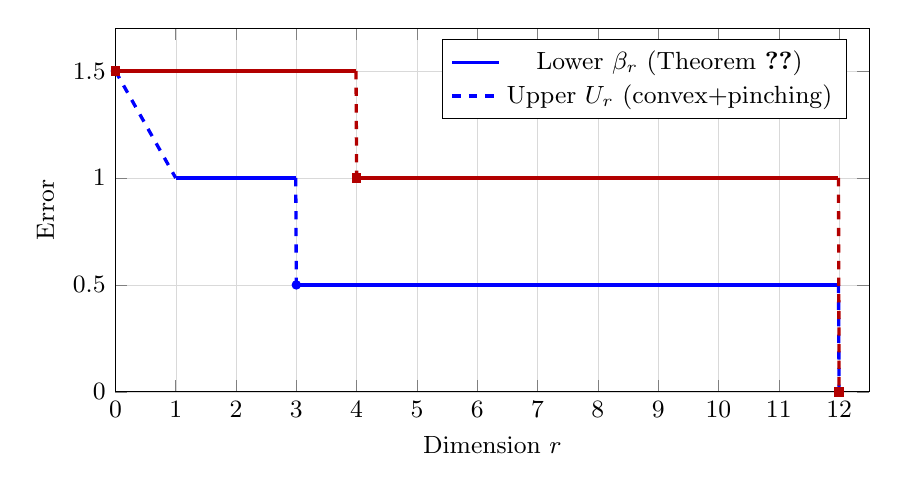
\begin{tikzpicture}
\begin{axis}[
    width=0.92\linewidth,
    height=6.2cm,
    xlabel={Dimension $r$},
    ylabel={Error},
    xmin=0, xmax=12.5,
    ymin=0, ymax=1.7,
    xtick={0,1,2,3,4,5,6,7,8,9,10,11,12},
    ytick={0,0.5,1,1.5},
    grid=both,
    grid style={line width=.1pt, draw=gray!30},
    legend pos=north east,
    legend style={font=\small},
    tick label style={font=\small},
    label style={font=\small}
]

\addplot[blue, very thick] coordinates {(1,1) (2.99,1)};
\addplot[blue, very thick, dashed] coordinates {(0,1.5) (1,1)};
\addplot[blue, very thick] coordinates {(3,0.5) (11.99,0.5)};
\addplot[blue, very thick, dashed] coordinates {(2.99,1) (3,0.5)};
\addplot[blue, very thick, dashed] coordinates {(11.99,0.5) (12,0)};
\addplot[blue, only marks, mark=*, mark size=1.5pt] coordinates {(0,1.5) (3,0.5) (12,0)};

\addplot[red!70!black, very thick] coordinates {(0,1.5) (3.99,1.5)};
\addplot[red!70!black, very thick] coordinates {(4,1) (11.99,1)};
\addplot[red!70!black, very thick, dashed] coordinates {(3.99,1.5) (4,1)};
\addplot[red!70!black, very thick, dashed] coordinates {(11.99,1) (12,0)};
\addplot[red!70!black, only marks, mark=square*, mark size=1.5pt] coordinates {(0,1.5) (4,1) (12,0)};
\legend{Lower $\beta_r$ (Theorem~\ref{thm:hierarchy}), Upper $U_r$ (convex+pinching)}
\end{axis}
\end{tikzpicture}
\caption{Qubit channels $d_A=d_B=2$, $D_{2,2}=12$: certified lower envelope $\beta_r$ (blue, $3/2$ at $r=0$ --- the exact constant-code width, where the envelopes coincide --- $1$ for $1\le r\le2$, $0.5$ for $3\le r\le11$, $0$ at $r\ge12$) and constructive upper envelope $U_r$ (red, $1.5$ for $0\le r\le3$, $1$ for $4\le r\le11$, $0$ at $12$). The drop at $r=4$ is balanced two-sector output pinching $Q_2(2)=2$, $r_{\rm out}=4$. The gap $0.5$ vs $1$ for $4\le r\le11$ is the undetermined positive width interval. For $r=3$ convex projection gives $2\cdot9/10=1.8$ but constant decoder $1.5$ is tighter.}
\label{fig:qubit-envelope}
\end{figure}

\section{Latent codes and physical programs}
\label{sec:codes}

The source bounds now pass to concrete code alphabets. Unrestricted
Euclidean and quantum-state codes provide the abstract benchmark.
Classical--quantum and reachable subsets then refine the relevant embedding
dimension, after which the decoder is restricted to a fixed physical
processor.

\subsection{Abstract latent and quantum-state codes}

\begin{theorem}[General latent-space channel bound]
\label{thm:general-latent}
Let $Y$ be Hausdorff and let the encoder $f:\Chan(A,B)\to Y$ be
continuous. If $r$ exceeds $\operatorname{coind}_{\mathbb Z_2}F_2(Y)$, then
every decoder $g:Y\to\TPHP(A,B)$ satisfies
\[
\sup_{\Phi\in\Chan(A,B)}
\|g(f(\Phi))-\Phi\|_\diamond
\geq\alpha_r(\Chan(A,B)).
\]
\end{theorem}

\begin{proof}
Take $K=\Chan(A,B)$ and $X=\TPHP(A,B)$ with the diamond metric in
Theorem~\ref{thm:intrinsic-latent}. Its coindex hypothesis is exactly the
one stated here, and its conclusion is the displayed inequality.
\end{proof}

\begin{theorem}[Quantum-state latent-code hierarchy]
\label{thm:compression}
Let $M$ be an $m$-dimensional Hilbert space, set $r=m^2-1$, and let
$\operatorname{Enc}:\Chan(A,B)\to\Sstate(M)$ be continuous. For every decoder $\operatorname{Dec}:\Sstate(M)\to\TPHP(A,B)$ (no regularity assumed), one has
\[
\sup_{\Phi\in\Chan(A,B)}
\|\operatorname{Dec}(\operatorname{Enc}(\Phi))-\Phi\|_\diamond
\geq\beta_r(A,B).
\]
Since channel-valued decoders form a subclass of $\TPHP(A,B)$-valued
decoders, the same lower bound applies a fortiori when the decoder is
required to output a channel. If the retained code is known to be
classical--quantum, the sharper affine dimension in
Proposition~\ref{prop:cq-code} should be used instead of the dimension of an
unrestricted density-operator space.
\end{theorem}

\begin{proof}
The trace-one affine hyperplane of $\Herm(M)$ has dimension $r=m^2-1$.
If $m=1$, the state space is a singleton, its deleted product has coindex
$-1$, and Theorem~\ref{thm:intrinsic-latent} applies with $r=0$.
Theorem~\ref{thm:full-state-antipodal} gives
$\alpha_0(\Chan(A,B))=1=\beta_0(A,B)$. If
$m\geq2$, affine coordinates inject $\Sstate(M)$ into $\mathbb R^r$;
Proposition~\ref{prop:euclidean-coindex} therefore bounds its deleted-product
coindex by $r-1$, and Theorem~\ref{thm:intrinsic-latent} again gives the
profile bound at index $r$. Theorem~\ref{thm:hierarchy} then yields
$\alpha_r(\Chan(A,B))\geq\beta_r(A,B)$ in both cases.
\end{proof}

\begin{proposition}[Exact abstract memory threshold]
\label{prop:memory-sharpness}
An exact continuous encoding into $\Sstate(M)$ followed by an unrestricted
channel-valued decoder exists if and only if
\[
m^2-1\geq D_{A,B}.
\]
Thus the least Hilbert-space dimension in this abstract model is
\[
m_{\min}=\left\lceil\sqrt{D_{A,B}+1}\right\rceil.
\]
\end{proposition}

\begin{proof}
Necessity follows from Proposition~\ref{prop:euclidean-threshold}: the depolarizing channel has positive-definite normalised Choi operator, hence is a relative interior point, so the channel body contains a positive relative ball.
For sufficiency, choose affine coordinates
$c:\operatorname{aff}\Chan(A,B)\to\mathbb R^{D_{A,B}}$ with
$c(\Omega_{A,B})=0$, and an injective linear map
$L:\mathbb R^{D_{A,B}}\to\Herm_0(M)$. Put
\[
C=\sup_\Phi\|L(c(\Phi))\|_\infty<\infty
\]
and choose $0<\varepsilon<1/(m\max\{1,C\})$. Then
\[
\operatorname{Enc}(\Phi)=\frac{I_M}{m}+\varepsilon L(c(\Phi)).
\]
The perturbation is traceless and has operator norm strictly below $1/m$ (strict inequality ensures positive definite, not merely semidefinite),
so every encoded operator is positive definite with trace one. The map is
a continuous affine injection into $\Sstate(M)$. Invert it set-theoretically
on its image and define the decoder arbitrarily elsewhere. No continuity or
physical implementability of this decoder is asserted.
\end{proof}

\begin{corollary}[Output-sized memory necessity]
\label{cor:accuracy-memory}
For a complete retained quantum-state alphabet $\Sstate(M)$, worst-case
error strictly below $1$ requires
\[
m\geq d_B.
\]
Worst-case error strictly below $\rhodep(A,B)$ requires
\[
m\geq\left\lceil\sqrt{D_{A,B}+1}\right\rceil.
\]
The first condition is only necessary. The second is also sufficient for
exact reconstruction in the abstract unrestricted-decoder model by
Proposition~\ref{prop:memory-sharpness}; no sufficiency for a fixed physical
processor is implied.
\end{corollary}

\begin{proof}
If $m<d_B$, then
$m^2-1\leq d_B^2-2$, so Theorem~\ref{thm:compression} gives error at least
one. If $m^2-1<D_{A,B}$, the same theorem gives error at least
$\rhodep(A,B)$. Taking contrapositives proves both claims.
\end{proof}

\subsection{Classical--quantum and reachable codes}

\begin{proposition}[Classical--quantum retained code]
\label{prop:cq-code}
Let the retained code consist of block-diagonal states
\[
\bigoplus_{j=1}^c\rho_j,
\qquad
\rho_j\geq0,
\qquad
\sum_j\Tr\rho_j=1,
\]
where the $j$th quantum block acts on a space of dimension $m_j$. Its
affine dimension is
\[
\sum_{j=1}^cm_j^2-1.
\]
Consequently, all Euclidean lower bounds apply with this value of $r$.
For equal block dimensions $m_j=m$, it reduces to $cm^2-1$.
\end{proposition}

\begin{proof}
A Hermitian block of size $m_j$ has real dimension $m_j^2$, so the direct
sum of all blocks has dimension $\sum_jm_j^2$. The total-trace-one
constraint removes one affine degree of freedom. The relative interior consists of those block-diagonal states $\bigoplus_j\rho_j$ for which every block $\rho_j$ is positive definite on its prescribed block space (block traces automatically positive); this set is nonempty, e.g., $\rho_j=I_{m_j}/(c m_j)$. Affine coordinates therefore give the required Euclidean
injection.
\end{proof}

\begin{corollary}[Classical--quantum output-size necessity]
\label{cor:cq-output-size}
For a complete retained classical--quantum alphabet with block dimensions
$m_1,\ldots,m_c$, worst-case error strictly below one requires
\[
\sum_{j=1}^cm_j^2\geq d_B^2.
\]
For equal block dimensions this becomes $cm^2\geq d_B^2$.
\end{corollary}

\begin{proof}
Proposition~\ref{prop:cq-code} embeds the complete alphabet into
$\mathbb R^{\sum_jm_j^2-1}$. If that dimension is at most $d_B^2-2$,
Theorem~\ref{thm:full-state-antipodal} and the Euclidean source--latent
obstruction give error at least one. Taking the contrapositive proves the
claim.
\end{proof}

\begin{definition}[Embedding dimension]
For a topological space $Z$, let
\[
\embdim(Z)=\inf\{s\in\mathbb N_0:Z\text{ admits a continuous injection into }
\mathbb R^s\},
\]
with value $+\infty$ if none exists.
\end{definition}

\begin{proposition}[Reachable-code refinement]
\label{prop:reachable}
Let $f:\Chan(A,B)\to Y$ be continuous and put
$Z=f(\Chan(A,B))$. If $\embdim(Z)\leq s$, then every decoder
$g:Y\to\TPHP(A,B)$ has worst-case diamond error at least
$\alpha_s(\Chan(A,B))$. The same lower bound holds for channel-valued
decoders.
\end{proposition}

\begin{proof}
Let $\iota:Z\to\mathbb R^s$ be a continuous injection. For every
$h:S^s\to\Chan(A,B)$, Borsuk--Ulam applied to
$\iota\circ f\circ h$ gives $u$ with
$\iota(f(h(u)))=\iota(f(h(-u)))$. Injectivity of $\iota$ implies that the
original latent codes coincide. The triangle-inequality argument in
Theorem~\ref{thm:intrinsic-latent} then gives the lower bound
$\alpha_s(\Chan(A,B))$ for every decoder $g$.
\end{proof}

\begin{proposition}[Structured latent-space coindex bounds]
\label{prop:structured-coindex}
The following statements hold.
\begin{enumerate}
\item A singleton has deleted-product coindex $-1$; a finite discrete space
with at least two points has coindex $0$; and
\[
\operatorname{coind}_{\mathbb Z_2}F_2(S^n)=n.
\]
\item If $n\geq1$, $Y$ contains a subset homeomorphic to a nonempty open
subset of an $n$-manifold, and $Y$ injects continuously into
$\mathbb R^s$, then
\[
n-1\leq\operatorname{coind}_{\mathbb Z_2}F_2(Y)\leq s-1.
\]
\item Let $\mathcal S_k(\mathbb C^m)$ denote the manifold of
density operators on $\mathbb C^m$ of rank exactly $k$ (i.e., $\{\rho\in\Sstate(\mathbb C^m):\operatorname{rank}\rho=k\}$), with its subspace topology. It is Hausdorff but noncompact (and not closed) for $1\le k<m$, and the coindex of Definition~\ref{def:coindex} requires only Hausdorffness. For pure
states and for $1\leq k<m$,
\begin{align*}
2m-3
&\leq\operatorname{coind}_{\mathbb Z_2}
F_2(\mathbb{CP}^{m-1})\leq m^2-2,\\
2mk-k^2-2
&\leq\operatorname{coind}_{\mathbb Z_2}
F_2(\mathcal S_k(\mathbb C^m))\leq m^2-2.
\end{align*}
For $m=2$, the pure-state value is exactly $2$.
\end{enumerate}
\end{proposition}

\begin{proof}
For a finite discrete space, an equivariant map from $S^0$ exists, whereas
connected spheres cannot map equivariantly into a discrete deleted product.
For $S^n$, the map $u\mapsto(u,-u)$ gives the lower bound and the standard
embedding into $\mathbb R^{n+1}$ gives the upper bound.

A nonempty open subset of an $n$-manifold, with $n\geq1$, contains a
coordinate ball $B^n$ and hence a small embedded $S^{n-1}$ as $\{x:\|x\|=\varepsilon\}$, giving the lower bound
in the second claim; Proposition
\ref{prop:euclidean-coindex} gives the upper bound. The pure-state manifold
has dimension $2m-2$, and the rank-$k$ stratum has dimension
$2mk-k^2-1$. Both lie in the $(m^2-1)$-dimensional affine space of
trace-one Hermitian matrices. Substitution gives the displayed bounds.
Finally, $\mathbb{CP}^1\simeq S^2$.
\end{proof}

\begin{remark}[Convex code spaces]
Proposition~\ref{prop:euclidean-coindex} gives the exact values
\[
\operatorname{coind}_{\mathbb Z_2}F_2(\Sstate(M))=m^2-2,
\qquad
\operatorname{coind}_{\mathbb Z_2}F_2(\Chan(A,B))=D_{A,B}-1,
\]
and
\[
\operatorname{coind}_{\mathbb Z_2}F_2(\operatorname{Rep}(A,B))=d_B^2-2.
\]
These equalities use convexity and nonempty relative interior; the nonconvex
spaces in Proposition~\ref{prop:structured-coindex} generally have only
upper and lower bounds.
\end{remark}

\subsection{Physical programmable processors}

The preceding results treat a density operator as an exact latent symbol. A
physical programmable decoder is more restrictive. Optimal asymptotic
program-cost scaling for approximate universal unitary programming is known
\cite{YangRennerChiribella2020}. The minimax quantities below isolate fixed
finite program dimension and give compactness, separation, and elementary
finite-packing consequences in diamond norm.

Let a fixed completely positive trace-preserving (CPTP) map
$\mathcal P:\Lin(M\otimes A)\to\Lin(B)$ induce
$\mathcal P_\rho(X)=\mathcal P(\rho\otimes X)$.

\begin{proposition}[Physical processor stability and scope]
\label{prop:processor}
For all program states,
\[
\|\mathcal P_\rho-\mathcal P_\sigma\|_\diamond
\leq\|\rho-\sigma\|_1.
\]
Since the lower bounds are universal over all decoders, they remain valid
when the decoder is restricted to a fixed physical processor. This does not
mean that the abstract zero-error decoder in
Proposition~\ref{prop:memory-sharpness} can be realized by such a processor:
no finite-dimensional deterministic processor exactly programs all unitary
channels on a nontrivial system.
\end{proposition}

\begin{proof}
For any state $\xi$ on a reference system tensored with the channel input
$A$, complete trace-norm contractivity gives
\[
\|(\id\otimes\mathcal P)((\rho-\sigma)\otimes\xi)\|_1
\leq\|\rho-\sigma\|_1\|\xi\|_1
=\|\rho-\sigma\|_1.
\]
Take the supremum over $\xi$. The exact universal-programming exclusion is
the no-programming theorem~\cite{NielsenChuang1997}.
\end{proof}

\begin{lemma}[Orthogonality of exact mixed program supports]
\label{lem:mixed-no-programming}
Suppose program states $\rho$ and $\sigma$ exactly implement two distinct
unitary channels through one deterministic processor. Then
\[
\operatorname{supp}\rho\perp\operatorname{supp}\sigma.
\]
\end{lemma}

\begin{proof}
Write $\rho=\sum_jp_j|a_j\rangle\langle a_j|$ with $p_j>0$. The induced
unitary channel is a convex combination of the channels programmed by the
pure states $|a_j\rangle$. A unitary channel is an extreme point of the convex set of
channels (its normalised Choi operator is rank one, and the rank-one states
are extreme), so every term of positive weight programs that same unitary.
The same holds for every eigenvector in the support of $\sigma$. The
pure-program no-programming theorem~\cite{NielsenChuang1997} makes pure
programs for distinct unitary channels orthogonal, proving orthogonality of
the two supports.
\end{proof}

\begin{theorem}[Positive finite-programming lower bound]
\label{thm:physical-programming-floor}
Let $H$ have dimension $d>1$ and let the complete retained program system
$M$ have fixed finite dimension $m$, with no additional side information
supplied to the processor. Define
\[
\gamma_{m,d}
=
\inf_{\mathcal P}
\sup_{\mathcal U\in\UChan(H)}
\min_{\rho\in\Sstate(M)}
\|\mathcal P_\rho-\mathcal U\|_\diamond,
\]
where the first infimum ranges over CPTP processors
$\mathcal P:\Lin(M\otimes H)\to\Lin(H)$. Then
\[
\gamma_{m,d}>0.
\]
Consequently, no number of queries used to prepare such an $m$-dimensional
program can make the worst-case physical programming error tend to zero while
$m$ remains fixed, because any finite-query encoder produces some program state in the fixed $m$-dimensional space and $\gamma_{m,d}$ already takes infimum over all such states and processors.
\end{theorem}

\begin{proof}
Via normalised Choi operators, the processors form a compact subset of a
common finite-dimensional matrix space. Indeed, the set of CPTP maps
$\Lin(M\otimes H)\to\Lin(H)$ is closed (Choi positivity and the linear
trace-preserving constraints) and bounded in trace, hence compact. The program-state and unitary-channel sets
are compact, and
\[
F(\mathcal P,\rho,\mathcal U)
=\|\mathcal P_\rho-\mathcal U\|_\diamond
\]
is jointly continuous. Define
\[
\omega(\mathcal P,\mathcal Q)
=\sup_{\rho,\mathcal U}
|F(\mathcal P,\rho,\mathcal U)-F(\mathcal Q,\rho,\mathcal U)|.
\]
Uniform continuity on the compact program--unitary product gives
$\omega(\mathcal P,\mathcal Q)\to0$ as $\mathcal Q\to\mathcal P$.
Taking a minimum over $\rho$ and then a maximum over $\mathcal U$ changes
a function by no more than its uniform perturbation. Therefore
\[
e(\mathcal P)
=\max_{\mathcal U\in\UChan(H)}
  \min_{\rho\in\Sstate(M)}F(\mathcal P,\rho,\mathcal U)
\]
is continuous. Hence $e$ attains its minimum over processors. If that
minimum were zero, one finite-dimensional processor would exactly implement
every unitary channel. Choosing $m+1$ distinct unitary channels would then
produce $m+1$ nonzero program states with pairwise orthogonal supports by
Lemma~\ref{lem:mixed-no-programming}, which is impossible in an
$m$-dimensional program space. Any program produced by a finite-query encoder is
among the states in the inner optimization, which proves the final claim.
\end{proof}

\begin{proposition}[Program-state separation]
\label{prop:program-separation}
Suppose a fixed processor approximates channels $\Phi_1,\ldots,\Phi_L$ with
program states $\rho_1,\ldots,\rho_L$ and error at most $\varepsilon$:
\[
\|\mathcal P_{\rho_j}-\Phi_j\|_\diamond\leq\varepsilon.
\]
Then
\[
\|\rho_i-\rho_j\|_1
\geq\|\Phi_i-\Phi_j\|_\diamond-2\varepsilon.
\]
\end{proposition}

\begin{proof}
The triangle inequality and Proposition~\ref{prop:processor} give
\[
\|\Phi_i-\Phi_j\|_\diamond
\leq2\varepsilon+
\|\mathcal P_{\rho_i}-\mathcal P_{\rho_j}\|_\diamond
\leq2\varepsilon+\|\rho_i-\rho_j\|_1.
\]
\end{proof}

\begin{theorem}[Packing lower bound for physical programming]
\label{thm:program-packing-rate}
Let $m\geq2$, put $n=m^2-1$, and suppose $L\geq2$ target unitary
channels in $\UChan(H)$ are pairwise diamond-separated by at least
$\Delta$; for $L=1$ the bound is trivial. Then
\[
\gamma_{m,d}
\geq
\max\left\{0,
\frac\Delta2-
\frac2{L^{1/n}-1}
\right\}.
\]
The same right-hand side also lower-bounds the continuous-assignment
quantity $\gamma^{\mathrm{cont}}_{m,d}$ defined below in
Proposition~\ref{prop:continuous-programming-floor}; once that quantity is defined, the bound applies to it as well because continuous program encoders form a subclass of all program assignments.
\end{theorem}

The proof is given in Appendix~\ref{app:program-packing-proof}.

\begin{corollary}[Explicit unitary-programming estimates]
\label{cor:explicit-programming}
The $d^2$ Weyl unitary channels are pairwise diamond-separated by two, so
for $m\geq2$,
\[
\gamma_{m,d}
\geq
\max\left\{0,
1-\frac2{d^{2/(m^2-1)}-1}
\right\}.
\]
For $m=d=2$, $n=3$, $L=4$, this general bound gives $1-2/(4^{1/3}-1)<0$, hence only the trivial bound $0$. A sharper qubit-specific packing argument using the Bloch sphere gives the following. For $m=1$, $\gamma_{1,d}\geq1$. For qubit targets and a qubit program,
\[
\gamma_{2,2}
\geq1-\frac12\sqrt{\frac83}.
\]
\end{corollary}

\begin{proof}
Fix the standard shift and phase operators $X$ and $Z$ on
$\mathbb C^d$. The $d^2$ operators $W_{a,b}=X^aZ^b$,
$0\leq a,b<d$, indexed by $\mathbb Z_d^2$, are Hilbert--Schmidt orthogonal ($\Tr(W_{a,b}^\dagger W_{c,d})=d\,\delta_{a,c}\delta_{b,d}$) and define $d^2$ distinct unitary channels up to global phase (global phase does not affect the channel). Hence maximally entangled
inputs perfectly distinguish their unitary channels. The first bound follows from
Theorem~\ref{thm:program-packing-rate}. A one-dimensional program gives one
fixed channel, which is at distance at least one from one of two perfectly
distinguishable targets.

For $m=d=2$, write four program states as
$\rho_i=(I+r_i\cdot\sigma)/2$, with Bloch vectors $r_i$ in the unit ball.
The Hermitian matrix
$\rho_i-\rho_j=(r_i-r_j)\cdot\sigma/2$ has eigenvalues
$\pm\|r_i-r_j\|_2/2$ because $(a\cdot\sigma)$ has eigenvalues $\pm\|a\|_2$, and hence
$\|\rho_i-\rho_j\|_1=\|r_i-r_j\|_2/2+\|r_i-r_j\|_2/2=\|r_i-r_j\|_2$. Therefore
\[
\sum_{i<j}\|r_i-r_j\|_2^2
=4\sum_i\|r_i\|_2^2-
 \left\|\sum_i r_i\right\|_2^2
\leq16.
\]
Among six pairs, one therefore has squared distance at most $8/3$.
Proposition~\ref{prop:program-separation} gives the last bound; equality in
the geometric estimate is attained by a regular tetrahedron.
\end{proof}

\begin{proposition}[Continuous physical-programming lower bound]
\label{prop:continuous-programming-floor}
Define
\[
\gamma^{\mathrm{cont}}_{m,d}
=
\inf_{\mathcal P}
\inf_{f\in C(\UChan(H),\Sstate(M))}
\sup_{\mathcal U\in\UChan(H)}
\|\mathcal P_{f(\mathcal U)}-\mathcal U\|_\diamond.
\]
Then
\[
\gamma^{\mathrm{cont}}_{m,d}
\geq\alpha_{m^2-1}(\UChan(H)).
\]
If $m^2-1\leq2\lfloor\log_2d\rfloor$, then
\[
\gamma^{\mathrm{cont}}_{m,d}\geq1.
\]
\end{proposition}

\begin{proof}
For fixed $\mathcal P$, the map
$g(\rho)=\mathcal P_\rho$ is a decoder from $\Sstate(M)$ to channels.
Affine coordinates inject $\Sstate(M)$ into $\mathbb R^{m^2-1}$, so the
source--latent obstruction applied to the continuous encoder $f$ gives the
first inequality. Corollary~\ref{cor:unitary-promise} gives the second.
Taking the two infima preserves both bounds.
\end{proof}

\begin{remark}[Continuous versus arbitrary program assignments]
The quantity $\gamma_{m,d}$ permits a discontinuous assignment of program
states, whereas $\gamma^{\mathrm{cont}}_{m,d}$ requires a continuous program
encoder. Compactness proves positivity of the former but does not determine
its value. Proposition~\ref{prop:program-separation} supplies the basic
metric input for quantitative packing estimates.
\end{remark}

Table~\ref{tab:resource-models} collects the decoder and retained-code
assumptions used by the abstract and operational statements. Its first four
rows summarize the models of this section; the final three preview the
query-generated encoders treated in Section~\ref{sec:adaptive}.

\begin{table}[t]
\centering
\small
\setlength{\tabcolsep}{4pt}
\begin{tabular}{p{3.2cm}p{4.0cm}p{3.3cm}p{3.2cm}}
\hline
Model & Complete retained code & Decoder model & Applicable statement\\
\hline
Euclidean latent code
& $\mathbb R^r$
& unrestricted
& fiber/profile bounds\\
Quantum-state alphabet
& $\Sstate(M)$, $r=m^2-1$
& unrestricted
& channel lower envelope\\
Classical--quantum code
& blocks $m_j$, $r=\sum_jm_j^2-1$
& unrestricted
& channel envelope with the complete code dimension\\
Physical program
& program state on $M$
& fixed CPTP processor
& $\gamma_{m,d}>0$; continuous-assignment profile bound\\
Deterministic $N$-query network
& complete final quantum--classical output
& unrestricted or physical
& bound uniform in finite $N$\\
Uniform postselection
& normalised success state, $p\geq p_0$
& as above
& same source bound on the success domain\\
Finite sampled transcript
& one sampled symbol from a $c$-element alphabet; its channel-dependent law $p(\cdot|\Phi)$ lies in
$\Sigma(T)\subseteq\mathbb R^{c-1}$ (transcript distribution), actual transcript sampled from that distribution
& randomized transcript decoder (Borel $Q_t$)
& collision lower bound $\alpha_{c-1}$; IC $N^{-1/2}$ upper bound with growing alphabet\\
\hline
\end{tabular}
\caption{Coding and reconstruction models. Classical transcripts and side
registers count as part of the complete retained code.}
\label{tab:resource-models}
\end{table}

\section{Adaptive query access}
\label{sec:adaptive}

The previous section constrains a code once its encoder is known to be
continuous. Here finite-query networks supply that continuity
operationally. The hybrid estimate first controls deterministic retained
states, after which the source bounds are applied to fixed final-code
alphabets and uniformly successful postselection. Finite sampled transcripts
are treated separately with both collision lower bounds and an explicit
reconstruction protocol.

\subsection{Deterministic networks and implementation sensitivity}

\begin{definition}[Deterministic finite-query network]
A deterministic $N$-query network is a causally ordered finite sequence of
CPTP interleaving maps with the unknown channel inserted in $N$ designated
slots. Finite ancillas, coherent controls, intermediate measurements, and
classically controlled operations are allowed. The complete final output
includes every classical outcome, quantum register, and side system available
to the decoder. If an outcome is discarded, the final code is the averaged
state resulting from that discard. Postselection is excluded unless stated
separately.
\end{definition}

\begin{figure}[t]
\hspace*{-8mm}
\centering
\resizebox{0.98\linewidth}{!}{
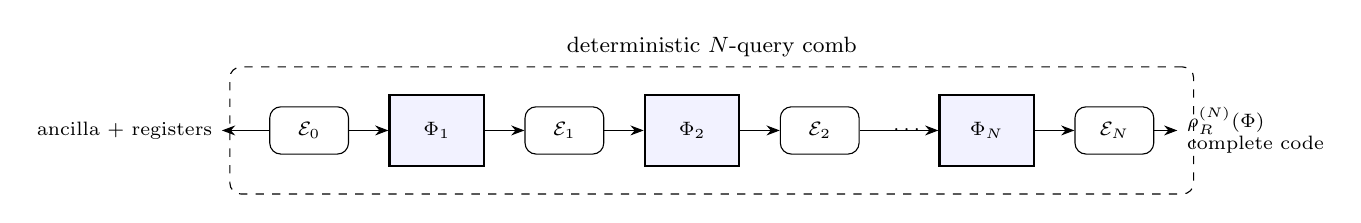
\begin{tikzpicture}[
  >=Stealth,
  box/.style={draw, rounded corners, minimum height=6mm, minimum width=10mm, align=center, font=\scriptsize},
  slot/.style={draw, thick, minimum height=9mm, minimum width=12mm, align=center, font=\scriptsize, fill=blue!5},
  every node/.style={font=\scriptsize}
]

\node[box] (E0) at (0,0) {$\mathcal E_0$};
\node[slot, right=5mm of E0] (Phi1) {$\Phi_1$};
\node[box, right=5mm of Phi1] (E1) {$\mathcal E_1$};
\node[slot, right=5mm of E1] (Phi2) {$\Phi_2$};
\node[box, right=5mm of Phi2] (E2) {$\mathcal E_2$};
\node at (E2.east) [right=3mm] {$\cdots$};
\node[slot, right=10mm of E2] (PhiN) {$\Phi_N$};
\node[box, right=5mm of PhiN] (EN) {$\mathcal E_N$};


\draw[->] (E0.west) -- ++(-6mm,0) node[left, font=\scriptsize] {ancilla + registers};
\draw[->] (E0) -- (Phi1);
\draw[->] (Phi1) -- (E1);
\draw[->] (E1) -- (Phi2);
\draw[->] (Phi2) -- (E2);
\draw[->] (E2) -- (PhiN);
\draw[->] (PhiN) -- (EN);
\draw[->] (EN) -- ++(8mm,0) node[right, align=left] {$\rho_R^{(N)}(\Phi)$\\complete code};


\begin{scope}[on background layer]
\node[draw, dashed, rounded corners, fit=(E0) (EN), inner sep=5mm, label=above:{\footnotesize deterministic $N$-query comb}] (comb) {};
\end{scope}
\end{tikzpicture}
}
\vspace{2mm}
\begin{minipage}{0.92\linewidth}
\footnotesize
\textbf{Complete code includes:} all quantum registers, classical outcomes, control bits, and side systems available to decoder. Discarding an outcome corresponds to averaging. Classical transcript $T\in\{1,\dots,c\}$ sampled from $p(\cdot|\Phi)\in\Sigma_{c-1}$ is part of $\rho_R^{(N)}$ when retained; its law is continuous in $\Phi$ (Proposition~\ref{prop:physical-continuity}). Postselection with $p(\Phi)\ge p_0>0$ keeps continuity after normalisation (Proposition~\ref{prop:postselection}).
\end{minipage}
\caption{Deterministic finite-query adaptive network as a quantum comb. The $N$ slots are filled with the unknown channel (or with slot-dependent channels $\Phi_j$, as in the heterogeneous-sensitivity Corollary~\ref{cor:heterogeneous-slots} stated below). All interleavings are fixed CPTP maps, possibly with coherent control and intermediate measurements. The final state $\rho_R^{(N)}$ is the complete retained code; any classical transcript, quantum memory $M$, or cq blocks $(m_j)$ is a function of it. Lower bounds $\beta_r$ depend only on $\operatorname{embdim}(f(\Chan))$ or $\operatorname{coind}F_2(Y)$, uniformly in $N$.}
\label{fig:comb-complete-code}
\end{figure}

Figure~\ref{fig:comb-complete-code} shows the complete retained code as the output of the comb. The following hybrid argument quantifies its sensitivity.



\begin{proposition}[Hybrid Lipschitz estimate]
\label{prop:physical-continuity}
Let $\rho_R^{(N)}(\Phi)$ be the complete final state produced by a
deterministic $N$-query network. Then
\[
\|\rho_R^{(N)}(\Phi)-\rho_R^{(N)}(\Psi)\|_1
\leq N\|\Phi-\Psi\|_\diamond.
\]
\end{proposition}

\begin{proof}
Order the slots causally. For $k=0,\ldots,N$, let $\rho^{(k)}$ be the
final state when the first $k$ slots use $\Phi$ and the remainder use
$\Psi$. For $k=1,\ldots,N$, adjacent hybrids use identical channels and
operations before slot $k$, so the joint state entering that slot is the
same. Replacing one channel changes the trace norm by at most
$\|\Phi-\Psi\|_\diamond$. This remains valid for every accumulated ancilla
including arbitrary classical registers because the diamond norm is already stabilized at a reference dimension
$d_A$~\cite{Watrous2018}, i.e., $\|\Phi-\Psi\|_\diamond=\sup_{\rho\in\Sstate(A_0\otimes A)}\|(id\otimes(\Phi-\Psi))(\rho)\|_1$ suffices for any extension. Subsequent deterministic CPTP maps contract trace norm. Therefore
\[
\|\rho^{(k)}-\rho^{(k-1)}\|_1
\leq\|\Phi-\Psi\|_\diamond,
\]
and summing over $k$ proves the claim.
\end{proof}

\begin{corollary}[Heterogeneous-slot implementation sensitivity]
\label{cor:heterogeneous-slots}
For two deterministic networks with the same interleaving maps and slot
channels $\Phi_1,\ldots,\Phi_N$ and
$\widetilde\Phi_1,\ldots,\widetilde\Phi_N$, respectively,
\[
\|\rho_R(\Phi_1,\ldots,\Phi_N)
-\rho_R(\widetilde\Phi_1,\ldots,\widetilde\Phi_N)\|_1
\leq
\sum_{j=1}^N\|\Phi_j-\widetilde\Phi_j\|_\diamond.
\]
If the reconstruction decoder is $L$-Lipschitz from trace norm to
diamond distance, the reconstructed maps differ by at most $L$ times the
same sum.
\end{corollary}

\begin{proof}
Form hybrids that replace the slot channels one at a time in causal order.
The diamond norm bounds the change at the replaced slot, and all subsequent
CPTP operations contract the trace norm. Summing the adjacent-hybrid bounds
proves the first claim; the decoder estimate is its Lipschitz consequence.
\end{proof}

\subsection{Uniform query bounds and postselection}

Let $\mathfrak C_N(M)$ denote the class of deterministic finite-dimensional
$N$-query networks whose complete retained output is a state on an
$m$-dimensional quantum system $M$. Separately, let
$\mathfrak C_N^{\mathrm{cq}}(m_1,\ldots,m_c)$ denote networks whose complete
retained output belongs to the classical--quantum alphabet with block
dimensions $m_1,\ldots,m_c$.

\begin{theorem}[Query-independent final-code bottleneck]
\label{thm:query-independent}
Set $r=m^2-1$. For every $N\geq1$, every
$\mathcal C^{(N)}\in\mathfrak C_N(M)$, and every unrestricted decoder from
$\Sstate(M)$ to $\TPHP(A,B)$, the worst-case error is at least
$\beta_r(A,B)$. Consequently,
\[
\inf_{N\geq1}
\inf_{\mathcal C^{(N)}\in\mathfrak C_N(M)}
\inf_{\operatorname{Dec}_N:\Sstate(M)\to\TPHP(A,B)}
\sup_{\Phi\in\Chan(A,B)}
\|\operatorname{Dec}_N(\rho_R^{(N)}(\Phi))-\Phi\|_\diamond
\geq\beta_r(A,B).
\]
The same lower bound applies to the limit inferior of any sequence of such
finite-query worst-case errors.
\end{theorem}

\begin{proof}
Proposition~\ref{prop:physical-continuity} gives continuity of every final
encoder. Apply Theorem~\ref{thm:compression}. The bound is independent of
$N$, so it survives all displayed infima and every limit inferior.
\end{proof}

\begin{corollary}[Query-independent classical--quantum code bound]
\label{cor:query-cq}
For a network in
$\mathfrak C_N^{\mathrm{cq}}(m_1,\allowbreak\ldots,\allowbreak m_c)$, set
\[
r_{\mathrm{cq}}=\sum_{j=1}^cm_j^2-1.
\]
Every unrestricted decoder from that complete retained alphabet has
worst-case error at least $\beta_{r_{\mathrm{cq}}}(A,B)$, uniformly in every
finite query count.
\end{corollary}

\begin{proof}
Proposition~\ref{prop:cq-code} gives the Euclidean embedding dimension of
the retained alphabet. The final-code map is continuous by
Proposition~\ref{prop:physical-continuity}; apply the same source--latent
argument as in Theorem~\ref{thm:query-independent}.
\end{proof}

\begin{proposition}[Uniformly successful postselection]
\label{prop:postselection}
Let $\sigma_R^{(N)}(\Phi)$ be the subnormalized success-branch state of a
finite-query instrument, and suppose
$p(\Phi)=\Tr\sigma_R^{(N)}(\Phi)\geq p_0>0$ for all channels considered.
Then the normalised conditional encoder is continuous and satisfies
\[
\left\|
\frac{\sigma_R^{(N)}(\Phi)}{p(\Phi)}
-
\frac{\sigma_R^{(N)}(\Psi)}{p(\Psi)}
\right\|_1
\leq\frac{2N}{p_0}\|\Phi-\Psi\|_\diamond.
\]
If the success condition holds on all of $\Chan(A,B)$ and the complete
normalised success output belongs to the same retained latent alphabet, the
bounds $\beta_r(A,B)$ apply unchanged. If it holds only on a promised
compact subset $K_0$, the same argument gives the source bound
$\alpha_r(K_0)$; the full channel-body bounds apply only when $K_0$ contains
the relevant antipodal sections.
\end{proposition}

\begin{proof}
A CP trace-nonincreasing map $\mathcal E$ is trace-norm contractive on
Hermitian operators, which suffices for the states appearing below. Indeed, if $X=X_+-X_-$ is the Jordan decomposition,
then positivity and trace-nonincreasingness give
\[
\|\mathcal E(X)\|_1
\leq\Tr\mathcal E(X_+)+\Tr\mathcal E(X_-)
\leq\Tr X_++\Tr X_-=\|X\|_1.
\]
After a slot is fixed in the hybrid argument, continuation along the chosen
success branch is CP and trace-nonincreasing. Hence
$\|\sigma(\Phi)-\sigma(\Psi)\|_1\leq
N\|\Phi-\Psi\|_\diamond$. For positive subnormalized states $\sigma,\tau$
with traces $p,q\geq p_0$,
\begin{align*}
\left\|\frac\sigma p-\frac\tau q\right\|_1
&\leq\frac{\|\sigma-\tau\|_1}{p}
+q\left|\frac1p-\frac1q\right|\\
&\leq\frac{2}{p_0}\|\sigma-\tau\|_1.
\end{align*}
Indeed,
$q|1/p-1/q|=|p-q|/p$ because $q|1/p-1/q|=|q/p-1|=|q-p|/p$, and $|p-q|=|\Tr\sigma-\Tr\tau|\le\|\sigma-\tau\|_1$, so $q|1/p-1/q|\le\|\sigma-\tau\|_1/p$, and
$p\geq p_0$.
\end{proof}

\subsection{Finite sampled transcripts}

A retained probability distribution is a deterministic point of a simplex,
whereas an observed transcript is a random variable. The first result below
bounds worst-source expected error from the dimension of the full transcript
simplex; the subsequent informationally complete construction supplies a
finite-sample upper bound.

\begin{definition}[Sampled-transcript reconstruction error]
Let $T$ be a finite transcript alphabet and let
$p:K\to\Delta(T)$ be a continuous stochastic encoder. For each
$t\in T$, let $Q_t$ be a Borel probability distribution on decoder outputs
in $X$ (if expectations infinite, inequality trivial). Define
\[
\mathcal E(x)
=\sum_{t\in T}p(t|x)
  \int_Xd(z,x)\,dQ_t(z).
\]
\end{definition}

\begin{theorem}[Worst-case sampled-transcript obstruction]
\label{thm:sampled-transcript}
If $|T|=c<\infty$, then every continuous stochastic encoder and every
possibly randomized transcript decoder satisfy
\[
\sup_{x\in K}\mathcal E(x)\geq\alpha_{c-1}(K).
\]
\end{theorem}

\begin{proof}
If any displayed expected error is infinite or not well-defined, the conclusion is immediate (inequality interpreted trivially).
Otherwise all integrals below are finite and well-defined. Identify the probability simplex
$\Delta(T)$ with a subset of $\mathbb R^{c-1}$. For any
$h:S^{c-1}\to K$, Borsuk--Ulam gives an
antipodal pair $x_+=h(u)$ and $x_-=h(-u)$ with the same transcript
distribution. For every transcript $t$ and decoder output $z$,
\[
d(z,x_+)+d(z,x_-)\geq d(x_+,x_-).
\]
Integrating first against $Q_t$ and then against the common transcript
distribution gives
\[
\mathcal E(x_+)+\mathcal E(x_-)
\geq d(x_+,x_-).
\]
Thus one expected error is at least half the antipodal separation. Taking
the supremum over $h$ proves the result.
\end{proof}

\begin{corollary}[Sampled channel transcript]
\label{cor:sampled-channel-transcript}
Let a finite-query protocol output one sampled transcript from an alphabet
of cardinality $c$, with transcript probabilities continuous in the unknown
channel. Every possibly randomized reconstruction rule satisfies
\[
\sup_{\Phi\in\Chan(A,B)}
\mathbb E_\Phi
\|\widehat\Phi_T-\Phi\|_\diamond
\geq\alpha_{c-1}(\Chan(A,B))
\geq\beta_{c-1}(A,B).
\]
In particular, the lower bound is one whenever $c\leq d_B^2-1$.
\end{corollary}

\begin{proof}
Apply Theorem~\ref{thm:sampled-transcript} with the channel body and diamond
distance, followed by Theorem~\ref{thm:hierarchy}.
\end{proof}

\begin{proposition}[One-query injective latent-state encoder]
\label{prop:one-query-injective}
Write $\Sigma_D=\{p\in\mathbb R^{D+1}:p_i\geq0,\ \sum_{i=0}^Dp_i=1\}$ for the $D$-dimensional probability simplex with $D+1$ vertices (i.e., probability distributions on $D+1$ symbols).
For every sufficiently small $\eta>0$, there is a one-query measurement (a POVM that is informationally complete for the channel affine hull, i.e.\ for the direction space $V_{A,B}$; cf.~\cite{Scott2006} for informationally complete measurements in general) whose outcome-probability map $\Phi\mapsto p(\Phi)\in\Sigma_{D_{A,B}}$, $p_i(\Phi)=\Tr(\widehat J_\Phi E_i)$, is a continuous affine injection from $\Chan(A,B)$ into the classical probability simplex. Equivalently, the averaged, pre-sampling classical output state $\sum_i p_i(\Phi)|i\rangle\langle i|$ lies in $\Sigma_{D_{A,B}}$ and its channel-to-state map is continuous, affine, and injective. A single run yields only a sampled outcome; the sampled version is treated in Theorem~\ref{thm:sampled-achievability}.
\end{proposition}

\begin{proof}
Choose a Hilbert--Schmidt orthonormal basis
$H_1,\ldots,H_{D_{A,B}}$ of the direction space $V_{A,B}$. Every $H_i$ is
traceless. For $0<\eta<1/((D_{A,B}+1)\sum_i\|H_i\|_\infty)$, the operators
\[
E_i=\frac{I_{A_0\otimes B}}{D_{A,B}+1}+\eta H_i
\quad(1\leq i\leq D_{A,B}),
\]
and
\[
E_0=\frac{I_{A_0\otimes B}}{D_{A,B}+1}
-\eta\sum_{i=1}^{D_{A,B}}H_i
\]
are positive: each perturbing operator has operator norm at most $\eta\sum_i\|H_i\|_\infty<1/(D_{A,B}+1)$, below the minimal eigenvalue $1/(D_{A,B}+1)$ of $I/(D_{A,B}+1)$. They sum to the identity and hence form a POVM.

Prepare $|\omega_A\rangle$, apply the unknown channel once, measure the
resulting normalised Choi state, and retain the classical output state with
probabilities
\[
p_i(\Phi)=\Tr(\widehat J_\Phi E_i).
\]
The map $\Phi\mapsto p(\Phi)$ is affine and continuous. If
$p(\Phi)=p(\Psi)$ and $X=\widehat J_\Phi-\widehat J_\Psi$, then
$X\in V_{A,B}$ and $\Tr X=0$. For $1\leq i\leq D_{A,B}$,
\[
0=\Tr(XE_i)=\eta\Tr(XH_i).
\]
Since the $H_i$ form a basis of $V_{A,B}$, this implies $X=0$ and
$\Phi=\Psi$. Thus the output-state encoder is injective.
\end{proof}

\begin{theorem}[Finite-sample channel reconstruction]
\label{thm:sampled-achievability}
Fix any admissible perturbation parameter $\eta>0$ for the POVM constructed
in Proposition~\ref{prop:one-query-injective} (any fixed $\eta$ with $0<\eta<1/((D_{A,B}+1)\sum_i\|H_i\|_\infty)$); the resulting constant below
depends on this choice and the statement is an existence statement. Repeat that one-query experiment independently
$N$ times. There is a channel-valued decoder from the sampled transcript
such that
\[
\sup_{\Phi\in\Chan(A,B)}
\mathbb E_\Phi
\|\widehat\Phi_N-\Phi\|_\diamond
\leq
\min\left\{2,\ \frac{d_A\sqrt{d_Ad_B}}{\eta\sqrt N}\right\}.
\]
The ordered raw transcript alphabet has cardinality
$(D_{A,B}+1)^N$. Because the decoder below uses only outcome counts, it may
instead retain the count vector, whose alphabet has cardinality
$\binom{N+D_{A,B}}{D_{A,B}}$.
\end{theorem}

\begin{proof}
Write
\[
\widehat J_\Phi-\widehat J_{\Omega_{A,B}}
=\sum_{i=1}^{D_{A,B}}x_i(\Phi)H_i.
\]
Since $\widehat J_{\Omega_{A,B}}$ is scalar and the $H_i$ are traceless,
\[
p_i(\Phi)=\frac1{D_{A,B}+1}+\eta x_i(\Phi)
\quad(1\leq i\leq D_{A,B}).
\]
Let $q_i$ be the empirical frequency of outcome $i$ and set
\[
y_i=\frac{q_i-1/(D_{A,B}+1)}{\eta}.
\]
Let $c(\Phi)=(x_i(\Phi))_{i=1}^{D_{A,B}}$ and let
$C=c(\Chan(A,B))$. Project $y$ orthogonally onto $C$, and decode the
projected point to a channel $\widehat\Phi_N$. Euclidean projection onto a
closed convex set is nonexpansive, so
\[
\|c(\widehat\Phi_N)-c(\Phi)\|_2
\leq\frac1\eta\|q_{1:D_{A,B}}-p_{1:D_{A,B}}(\Phi)\|_2.
\]
For $\Delta=\widehat\Phi_N-\Phi$, Lemma~\ref{lem:choi-upper} gives $\|\Delta\|_\diamond\le\|\Tr_B|J_\Delta|\|_\infty$, and $\|\Tr_B|J_\Delta|\|_\infty\le\|\Tr_B|J_\Delta|\|_1\le\|J_\Delta\|_1$ because operator norm $\le$ trace norm and partial trace is trace-norm contractive. Cauchy--Schwarz then gives
\begin{align*}
\|\Delta\|_\diamond
&\leq\|\Tr_B|J_\Delta|\|_\infty
\leq\|J_\Delta\|_1\\
&\leq d_A\sqrt{d_Ad_B}\,\|\widehat J_\Delta\|_2
=d_A\sqrt{d_Ad_B}\,
\|c(\widehat\Phi_N)-c(\Phi)\|_2.
\end{align*}
The multinomial covariance identity gives
\[
\mathbb E_\Phi
\|q_{1:D_{A,B}}-p_{1:D_{A,B}}(\Phi)\|_2^2
=\frac1N\left(
\sum_{i=1}^{D_{A,B}}p_i(\Phi)
-\sum_{i=1}^{D_{A,B}}p_i(\Phi)^2
\right)
\leq\frac1N.
\]
Jensen's inequality proves the decay bound, and the minimum with $2$ is
admissible because the channel body has diamond diameter $2$ for $d_B>1$
(Section~\ref{sec:replacement-unitary}), so the displayed estimate is
non-vacuous for every $N$; the decay is the asymptotic content. The decoder is defined as above on the encoder image (count vectors) and set to the fixed channel $\Omega_{A,B}$ outside that image; no regularity is required. Concentration follows from Hoeffding's inequality, and sample-optimal state tomography bounds are given in~\cite{HaahEtAl2017}.
\end{proof}

\begin{remark}[Latent states and sampled outcomes]
Proposition~\ref{prop:one-query-injective} concerns the averaged classical
state and the unrestricted decoder model. One execution supplies one
sampled outcome, not the exact probability vector. Theorem
\ref{thm:sampled-achievability} gives the corresponding operational
finite-sample statement; its growing transcript alphabet is consistent with
Theorem~\ref{thm:sampled-transcript}.
\end{remark}

\begin{remark}[Sampled transcripts and retained information]
This is a worst-channel expected-error statement, not a Bayes-average bound
for an arbitrary nonatomic prior. If a length-$N$ transcript uses a
$c$-symbol alphabet, the complete transcript alphabet can have up to $c^N$
values; if only a statistic with $L$ values is retained, $L-1$ is the
relevant simplex dimension. The decoder receives only that complete
retained code and has no subsequent access to the unknown channel. Every
classical transcript, quantum register, reference system, or side register
available to it is part of the code. A sampled transcript with
expected-error performance is a probabilistic model and is not identified
with the deterministic average output state.
\end{remark}

\begin{remark}[Continuity is essential]
Without encoder regularity, a set-theoretic injection of the channel body
into another continuum, followed by its inverse on the image, gives exact
reconstruction. The obstruction is therefore topological rather than
cardinality-based: continuity of the encoder is indispensable, while the
decoder may remain unrestricted.
\end{remark}

\begin{remark}[Continuity versus the Lipschitz constant]
Continuity alone activates the exact antipodal collision and the topological
lower bound. The factor $N$ quantifies implementation sensitivity but does not
weaken the lower bound as $N$ grows. It becomes relevant in noisy-code or
Lipschitz-decoder variants such as Theorem~\ref{thm:stable-obstruction}.
\end{remark}

\section{Conclusion and open problems}
\label{sec:conclusion}

Encoder-continuous reconstruction admits an exact fiber-radius formulation. The antipodal profile quantifies source geometry and the deleted-product coindex quantifies latent collision topology. The replacement family, the observable sphere, and their join provide the maximal lower bound $1$ through index $L_{A,B}$; the Clifford construction extends perfect separation to unitary channels. Across the remaining subcritical dimensions the globally optimal centred ball and the full-direction section give the certified lower bound $\gamma_{A,B}=\max\{\rhodep(A,B),1/d_A\}$ up to the affine dimension $D_{A,B}=d_A^2(d_B^2-1)$, which is the exact threshold for zero-error continuous encoding with unrestricted decoder. The $n$-outcome instrument versions of these results appear in Ref.~\cite{CompanionInstruments}. The depolarizing channel is an optimal constant decoder with exact covering radius $2-\rhodep(A,B)$. The lower envelope is complemented by constructive upper envelopes from convex projection and balanced input/output pinching, as illustrated in Figure~\ref{fig:qubit-envelope} and Figure~\ref{fig:replacement-join}, bracketing the unknown positive widths; at $r=0$ the two envelopes meet at the exact constant-code width. For abstract quantum-state codes the bounds imply $m\ge d_B$ is necessary for error below one and $m^2-1\ge D_{A,B}$ is necessary and sufficient for exact encoding.

The Euclidean zero-error threshold is not a universal-programming threshold. Every deterministic finite-query adaptive network, equivalently a finite quantum comb, induces a continuous final code containing all classical and quantum side information (Figure~\ref{fig:comb-complete-code}); the same dimensional bottlenecks hold uniformly in the query count, for uniformly successful postselection, and for finite sampled transcripts. A one-query informationally complete measurement yields a continuous injective encoding at the affine threshold, and repeated sampling yields a channel-valued estimator with expected error $O(N^{-1/2})$. These results isolate final representational dimension as the obstruction, distinct from tomography sample complexity and from fixed-processor programming limits.

Several concrete problems remain:
\begin{enumerate}
\item determine the exact positive widths
$\widetilde\delta_r^\diamond(A,B)$ and $\delta_r^\diamond(A,B)$ for
$0<r<D_{A,B}$ (for $d_A=1$, the channel-level instance of the flat-widths problem of
Ref.~\cite{CompanionInstruments} is settled in the negative direction: the flat value
$\delta_r^\diamond=1$ fails at the bottom index for $d_B\ge5$ and, more generally,
at every $r\le(d_B-3)/2$ within $1\le r\le d_B^2-2$, by the coordinate-flag median
matching and topological Tverberg bounds of the companion --- at $d_A=1$ the diamond
norm on channel differences is the trace norm on output states, so the channel widths
coincide with the one-outcome instrument widths; and the companion's equal-value-basis theorem closes those two cases as well: the flat
value fails for every $d_B\ge3$ at the bottom index, with $\delta_1^\diamond\ge4/3$ ---
the qutrit channel state space exactly at $4/3$ and the ququart in $[4/3,\,3/2]$ --- and, at the second index, the companion's plane-valued extension of the equal-value-basis theorem likewise bounds $\delta_2^\diamond\ge4/3$ for every $d_B\ge3$, the qutrit again exactly at $4/3$ --- the cyclic flag quotient underlying that extension sits between the complete flag manifold and the symmetric-group unordered quotients whose cohomology is computed in Refs.~\cite{GuerraJana2025,GuerraJanaMaiti2025});
\item determine the exact perfect-separation indices $\pi(A,B)$ and
$\pi_{\mathrm U}(d)$ of Corollary~\ref{cor:perfect-separation-indices}
within the proved lower and upper ranges;
\item determine exact deleted-product coindices of structured nonconvex latent
spaces beyond the patch and embedding bounds proved here;
\item determine whether the optimal Chebyshev centre $\Omega_{A,B}$ is unique;
\item sharpen the explicit physical-programming packing bounds and develop
Bayes-risk or infinite-transcript formulations beyond the finite-alphabet
worst-case theorem.
\end{enumerate}

\section*{Declarations}
The author declares no funding and no competing interests. No datasets were generated or analysed.

\appendix
\section{Technical proofs}
\label{app:technical-proofs}

The appendix provides the complete matrix and volume proofs for the
full-body radius and covering results, the fixed-marginal and programming
estimates, and the structured partition and Clifford constructions.

\subsection{Exact all-dimensional centred in-radius}
\label{app:exact-inradius-proof}

\begin{proof}[Proof of Theorem~\ref{thm:exact-inradius}]
Let $s=\min\{d_A,d_B\}$. First consider an arbitrary nonzero
Hermiticity-preserving, trace-annihilating map $\Delta$, put
$X=\widehat J_\Delta$, and let
\[
\lambda=\lambda_{\max}(-X).
\]
Choose a unit vector $|v\rangle$ satisfying $X|v\rangle=-\lambda|v\rangle$.
Let $S\subseteq A_0$ be the support of
$\Tr_B|v\rangle\langle v|$ and set $b=\dim S$. The Schmidt rank of
$|v\rangle$ is $b$, so $b\leq s$.

Choose an orthonormal basis of $S$ and use the basis-conjugate subspace of
$A$ under the fixed identification $A_0\simeq A$. On these two subspaces
let
\[
|\omega_S\rangle
=\frac1{\sqrt b}\sum_{j=1}^b|j\rangle_{A_0}|j\rangle_A.
\]
If $P_S$ is the projection onto $S$, then the normalised-Choi convention
gives
\[
Y:=(\id_{A_0}\otimes\Delta)
(|\omega_S\rangle\langle\omega_S|)
=\frac{d_A}{b}(P_S\otimes I_B)X(P_S\otimes I_B).
\]
The operator $Y$ is Hermitian and traceless because $\Delta$ is
trace-annihilating. Since $|v\rangle\in S\otimes B$,
\[
\langle v|Y|v\rangle=-\frac{d_A}{b}\lambda.
\]
For a traceless Hermitian operator $Y=Y_+-Y_-$, $\Tr Y_+=\Tr Y_-=\frac12\|Y\|_1$ and for any unit vector $|v\rangle$, $\langle v|Y|v\rangle\ge -\|Y_-\|_\infty\ge -\Tr Y_- = -\frac12\|Y\|_1$. Hence
\[
\|Y\|_1
\geq-2\langle v|Y|v\rangle
=\frac{2d_A}{b}\lambda
\geq\frac{2d_A}{s}\lambda.
\]
Because $|\omega_S\rangle\langle\omega_S|$ is an admissible input in the
diamond-norm optimization,
\[
\|\Delta\|_\diamond\geq\|Y\|_1.
\]
Therefore
\[
\lambda_{\max}(-\widehat J_\Delta)
\leq\frac{s}{2d_A}\|\Delta\|_\diamond,
\]
and consequently $\Gamma_{A,B}\leq s/(2d_A)$.

For the matching witness, choose an $s$-dimensional subspace $S_A\subseteq A$
and two isometries $V_0,V_1:S_A\to B$ satisfying
$\Tr(V_0^\dagger V_1)=0$. If $s=1$, the standing assumption $d_B>1$
allows two orthogonal output unit vectors. If $s\geq2$, take
$V_1=V_0U$ for a traceless unitary $U$ on $S_A$.
Let
\[
|v_j\rangle=(I\otimes V_j)|\omega_{S_A}\rangle,
\qquad P_j=|v_j\rangle\langle v_j|,
\quad j=0,1.
\]
Then $P_0P_1=0$ and
\[
\Tr_BP_0=\Tr_BP_1=\frac{P_{S_A}}s.
\]
Define completely positive trace-nonincreasing maps
\[
\mathcal E_j(Z)=V_jP_{S_A}ZP_{S_A}V_j^\dagger.
\]
For every input operator $Z$,
$\Tr\mathcal E_j(Z)=\Tr(P_{S_A}Z)$; hence every scalar multiple of
$\mathcal E_1-\mathcal E_0$ is trace-annihilating. Each $\mathcal E_j$ has
diamond norm at most one. A maximally entangled input on $S_A$
produces the orthogonal pure outputs $P_0$ and $P_1$, so
\[
\|\mathcal E_1-\mathcal E_0\|_\diamond=2.
\]
Moreover,
\[
\widehat J_{\mathcal E_j}=\frac{s}{d_A}P_j.
\]
Thus the map
\[
\widetilde\Delta=\frac12(\mathcal E_1-\mathcal E_0)
\]
has diamond norm one and normalised Choi operator
\[
\widehat J_{\widetilde\Delta}
=\frac{s}{2d_A}(P_1-P_0).
\]
It follows that
\[
\lambda_{\max}(-\widehat J_{\widetilde\Delta})
=\frac{s}{2d_A},
\]
which proves $\Gamma_{A,B}=s/(2d_A)$. Proposition~\ref{prop:inradius-variational}
then yields
\[
\rho_\diamond(\Omega_{A,B})
=\frac{1}{d_Ad_B\Gamma_{A,B}}
=\frac{2}{d_Bs}.
\]
\end{proof}

\subsection{Exact Chebyshev covering radius}
\label{app:chebyshev-radius-proof}

\begin{proof}[Proof of Theorem~\ref{thm:exact-chebyshev-radius}]
Let $s=\min\{d_A,d_B\}$. Recall the diamond norm is already achieved with a reference system of dimension $d_A$, so we may assume $r=\operatorname{rank}\rho_R\le d_A$. A bipartite state $\sigma_{RB}$ with marginal
$\rho_R$ and $r=\operatorname{rank}\rho_R$ satisfies
\[
\sigma_{RB}\leq k\,\rho_R\otimes I_B,
\qquad
k=\min\{r,d_B\}.
\]
To prove this, restrict $R$ to the support of $\rho_R$ and set, with $\rho_R^{-1/2}$ denoting the Moore-Penrose inverse on its support,
\[
Z=(\rho_R^{-1/2}\otimes I_B)\sigma_{RB}
  (\rho_R^{-1/2}\otimes I_B).
\]
If $\sigma_{RB}=0$ then $\rho_R=0$ and the claim is immediate, so assume $\sigma_{RB}\neq0$. Then $Z\geq0$ and $\Tr_BZ=I_R$. With the column-vectorization convention of Section~\ref{sec:geometry},
$|K\rangle\rangle=\sum_{a,b}K_{ba}|a\rangle_R\otimes|b\rangle_B$, so that
$\Tr_B|K\rangle\rangle\langle\langle K|=K^\dagger K$ and
$\langle\langle V|K\rangle\rangle=\Tr(V^\dagger K)$, write
$Z=\sum_\alpha|K_\alpha\rangle\rangle
\langle\langle K_\alpha|$, where the condition $\Tr_BZ=I_R$ is equivalent to $\sum_\alpha K_\alpha^\dagger K_\alpha=I_R$. Let a unit vector
$|v\rangle$ of Schmidt rank $b\leq k$ correspond to a matrix
$V:R\to B$ with $\Tr(V^\dagger V)=1$. Then
$\operatorname{rank}V=b$. For each $\alpha$, the
matrix $K_\alpha V^\dagger$ has rank at most $b$. The elementary
rank--trace inequality
$|\Tr M|^2\leq\operatorname{rank}(M)\Tr(MM^\dagger)$, obtained by
Cauchy--Schwarz on the support of $M$ (write $M$ via SVD $M=\sum_{i=1}^{\operatorname{rank}M}s_i|u_i\rangle\langle w_i|$, then $|Tr M|^2\le \operatorname{rank}M\sum s_i^2|\langle w_i|u_i\rangle|^2\le \operatorname{rank}M\,Tr(MM^\dagger)$), therefore gives
\[
|\Tr(V^\dagger K_\alpha)|^2
=|\Tr(K_\alpha V^\dagger)|^2
\leq b\,\Tr(VK_\alpha^\dagger K_\alpha V^\dagger).
\]
Consequently,
\begin{align*}
\langle v|Z|v\rangle
&=\sum_\alpha|\langle v|K_\alpha\rangle\rangle|^2\\
&\leq b\,\Tr\left(
V\left(\sum_\alpha K_\alpha^\dagger K_\alpha\right)V^\dagger
\right)
=b\leq k.
\end{align*}
Thus $Z\leq kI$, which proves the domination inequality. Since
$r\leq d_A$, it follows that
\[
\sigma_{RB}
\leq d_Bs\left(\rho_R\otimes\frac{I_B}{d_B}\right).
\]

Both $\sigma_{RB}=(\id_R\otimes\Phi)(\xi_{RA})$ and $\tau=\xi_R\otimes I_B/d_B$ have trace one since $(\id_R\otimes\Phi)$ is itself a channel. If states $\rho$ and $\tau$ satisfy $\rho\leq K\tau$, let $P$ be the
positive spectral projection of $\rho-\tau$ and put
$a=\Tr(P\rho)$ and $b=\Tr(P\tau)$. Then $a\leq Kb$ because $P\rho P\le K P\tau P$, and $a\leq1$, so
\[
\frac12\|\rho-\tau\|_1=a-b
\leq a\left(1-\frac1K\right)
\leq1-\frac1K.
\]
Applying this with $K=d_Bs$ to
$\sigma_{RB}=(\id_R\otimes\Phi)(\xi_{RA})$ and
$\tau=\xi_R\otimes I_B/d_B$ yields
\[
\|\Phi-\Omega_{A,B}\|_\diamond
\leq2\left(1-\frac1{d_Bs}\right).
\]

For the reverse inequality, choose an $s$-dimensional subspace
$S\subseteq A$, an isometry $V:S\to B$, and a state $\tau$ on $B$. With
$P_S$ the subspace projection, define the channel
\[
\Phi(X)=VP_SXP_SV^\dagger+
\Tr[(I_A-P_S)X]\,\tau.
\]
A maximally entangled input of Schmidt rank $s$ supported on $S$ produces a
pure maximally entangled output, whereas the depolarizing channel produces
$I_{R_sB}/(sd_B)$. Their trace norm is
\[
2\left(1-\frac1{sd_B}\right).
\]
Theorem~\ref{thm:depolarizing-chebyshev} then gives the asserted constant-code
equalities.
\end{proof}

\subsection{One-sided twirling with a fixed marginal}
\label{app:fixed-marginal-proof}

\begin{proof}[Proof of Proposition~\ref{prop:fixed-marginal-chebyshev}]
For an operator $Y$ on $B_1\otimes B_2$, one-sided Haar twirling gives
\[
\int_{\mathrm U(B_2)}
(I_{B_1}\otimes V)Y(I_{B_1}\otimes V^\dagger)\,dV
=
\Tr_{B_2}(Y)\otimes\frac{I_{B_2}}{d_{B_2}}.
\]
Indeed, expand $Y$ in matrix units on $B_1$ and apply the scalar Haar-twirl
identity to every $B_2$ block.

Let $R_K(\Psi)=\sup_{\Phi\in K}\|\Phi-\Psi\|_\diamond$ on the affine class
of centres with marginal $\Lambda$. Invariance of $K$ makes $R_K$ invariant
under post-composition by the conjugation channel
$\operatorname{id}_{B_1}\otimes\mathcal C_V$, and $R_K$ is convex. The
one-sided twirl of every admissible centre is
\[
X\longmapsto\Lambda(X)\otimes\frac{I_{B_2}}{d_{B_2}}=\Phi_0(X).
\]
Jensen's inequality therefore gives $R_K(\Phi_0)\leq R_K(\Psi)$ for every
admissible centre.
\end{proof}

\subsection{Physical-programming packing bound}
\label{app:program-packing-proof}

\begin{proof}[Proof of Theorem~\ref{thm:program-packing-rate}]
Fix an arbitrary processor $\mathcal P$ and put
\[
e(\mathcal P)=
\sup_{\mathcal U\in\UChan(H)}
\min_{\rho\in\Sstate(M)}
\|\mathcal P_\rho-\mathcal U\|_\diamond.
\]
Choose target channels $\Phi_1,\ldots,\Phi_L$ with pairwise diamond distance
at least $\Delta$. Compactness of the program-state space gives, for every
target, a minimizing program state $\rho_i$ (minimum attained because $\Sstate(M)$ is compact and $\rho\mapsto\|\mathcal P_\rho-\mathcal U\|_\diamond$ is continuous, indeed $\|\mathcal P_\rho-\mathcal P_\sigma\|_\diamond\le\|\rho-\sigma\|_1$), and its error is at most
$e(\mathcal P)$. Proposition~\ref{prop:program-separation} therefore gives
\[
\|\rho_i-\rho_j\|_1\geq
\eta:=\Delta-2e(\mathcal P).
\]
If $\eta=\Delta-2e(\mathcal P)\leq0$, then
$e(\mathcal P)\geq\Delta/2$ and the asserted lower bound is immediate (with positive-part convention $\max\{0,\cdot\}$).
Assume $\eta>0$ and translate the affine space of trace-one Hermitian
matrices by $\rho_1$. It is a real
normed space of dimension $n=m^2-1$. All translated program states lie in
the trace-norm ball of radius two, and the open balls of radius $\eta/2$
about them are disjoint. These balls lie in the ball of radius
$2+\eta/2$ about the origin. Fix any Lebesgue measure on this
$n$-dimensional real vector space. Its norm balls scale in volume as the
$n$th power of the radius up to a constant depending on the norm shape which cancels in the ratio, i.e., $\mathrm{Vol}(B(0,r))=r^n\mathrm{Vol}(B(0,1))$, so
\[
L\left(\frac\eta2\right)^n
\leq\left(2+\frac\eta2\right)^n.
\]
Hence
\[
\eta\leq\frac4{L^{1/n}-1}.
\]
Substituting $\eta=\Delta-2e(\mathcal P)$ and rearranging gives
\[
e(\mathcal P)\geq
\frac\Delta2-\frac2{L^{1/n}-1}.
\]
The processor was arbitrary, so taking its infimum proves the claimed bound
for $\gamma_{m,d}$. Continuous program encoders form a subclass of all
program assignments, so the same estimate applies to them.
\end{proof}

\subsection{Structured partition sections}
\label{app:partition-sections}

\begin{proposition}[Orthogonal-block join]
\label{prop:join}
Let $B=\bigoplus_{i=1}^{\ell}B_i\oplus B_\perp$. Suppose
$h_i:S^{r_i}\to\Sstate(B_i)$ are continuous and
\[
\|h_i(u)-h_i(-u)\|_1\geq2\rho_i.
\]
Then there is a continuous
\[
H:S^{\sum_i r_i+\ell-1}\to\Sstate(B)
\]
whose antipodal trace norm is at least
$2\min_i\rho_i$.
\end{proposition}

\begin{proof}
Regard the domain sphere as the unit sphere in
$\bigoplus_i\mathbb R^{r_i+1}$. For $y=(y_1,\ldots,y_\ell)$, put
$\lambda_i=\|y_i\|_2^2$ and, when $y_i\neq0$,
$u_i=y_i/\|y_i\|_2$. Define the $i$th block of $H(y)$ to be
$\lambda_i h_i(u_i)$, and set it to zero when $y_i=0$. The latter extension
is continuous because the block trace norm is $\lambda_i$. Since
$\sum_i\lambda_i=1$, $H(y)$ is a state. Orthogonality of the blocks gives
\begin{align*}
\|H(y)-H(-y)\|_1
&=\sum_i\lambda_i\|h_i(u_i)-h_i(-u_i)\|_1\\
&\geq2\min_i\rho_i.
\end{align*}
\end{proof}

\begin{theorem}[Partitioned replacement sections]
\label{thm:partition}
Let $b_1,\ldots,b_\ell\geq2$ satisfy $\sum_i b_i\leq d_B$, and put
\[
R_{\mathrm J}=\sum_i(b_i^2-1)-1,
\]
the block-join index. Then
\[
\alpha_r(\Chan(A,B))=1,
\qquad0\leq r\leq R_{\mathrm J}.
\]
\end{theorem}

\begin{proof}
On a block of dimension $b_i\geq2$, the Jordan construction in the proof of
Theorem~\ref{thm:full-state-antipodal}, restricted to
$\Herm_0(B_i)\subseteq\Herm_0(B)$, gives a continuous map
$h_i:S^{b_i^2-2}\to\Sstate(B_i)$ whose antipodes have orthogonal supports,
hence trace norm $2$. Proposition~\ref{prop:join} produces a sphere of dimension
\[
\sum_i(b_i^2-2)+\ell-1
=\sum_i(b_i^2-1)-1=R_{\mathrm J}
\]
with antipodal trace norm $2$. Replacement channels preserve this
distance by Lemma~\ref{lem:replacement}, so the antipodal separation in
diamond distance is $2$; dividing by two gives the profile value one on
this sphere. Restriction to coordinate equators gives every smaller $r$,
and the diameter bound supplies the reverse inequality.
\end{proof}

\begin{corollary}[Block-size envelope]
\label{cor:block-envelope}
Fix a block-size cap $2\leq c\leq d_B$ and write $d_B=mc+t$, $0\leq t<c$. Set
\[
R_{\mathrm J}(c)=
\begin{cases}
m(c^2-1)-1,&t=0\text{ or }t=1,\\
m(c^2-1)+t^2-2,&2\leq t<c.
\end{cases}
\]
Then
\[
\alpha_r(\Chan(A,B))=1,
\qquad0\leq r\leq R_{\mathrm J}(c).
\]
In particular, for $c=2$ (two-dimensional blocks),
\[
\alpha_r(\Chan(A,B))=1
\quad\text{for}\quad
0\leq r\leq3\left\lfloor\frac{d_B}{2}\right\rfloor-1.
\]
\end{corollary}

\begin{proof}
If $t=0$ or $t=1$, use $m$ blocks of size $c$ and leave the possible
one-dimensional remainder unused. Theorem~\ref{thm:partition} then gives
$R_{\mathrm J}(c)=m(c^2-1)-1$. If $2\leq t<c$, add one block of size $t$, giving
$R_{\mathrm J}(c)=m(c^2-1)+(t^2-1)-1$. For $c=2$ this is $3\lfloor d_B/2\rfloor-1$ for both parities of $d_B$. Theorem~\ref{thm:partition} gives the value one
on this range, and the diameter bound supplies the reverse inequality.
\end{proof}

\begin{proposition}[Optimization within a block-size constraint]
\label{prop:partition-optimization}
Fix a block-size cap $2\leq c\leq d_B$. Among all partitions with
$2\leq b_i\leq c$ and $\sum_i b_i\leq d_B$, the largest value of
$\sum_i(b_i^2-1)-1$ is $R_{\mathrm J}(c)$ from
Corollary~\ref{cor:block-envelope}.
\end{proposition}

\begin{proof}
It is enough to maximise
$F=\sum_i(b_i^2-1)$, because the final subtraction by one is fixed.
A maximizing partition leaves at most one output dimension unused: if at
least two dimensions were unused, one could add a block of size between two
and $c$, strictly increasing $F$.

We next show that a maximizer has at most one block smaller than $c$.
Suppose two such blocks have sizes $2\leq a\leq b<c$. If $a+b\leq c$,
replace them by one block of size $a+b$; the change in $F$ is
\[
(a+b)^2-1-(a^2-1)-(b^2-1)=2ab+1>0.
\]
If $a+b=c+1$, replace them by one $c$-block and leave one dimension unused;
the change is
\[
c^2-1-(a^2-1)-(b^2-1)=2(a-1)(b-1)>0.
\]
If $a+b\geq c+2$, replace them by blocks of sizes $c$ and $a+b-c$, the
latter lying between two and $c-2$. The change is
\[
(c^2-1)+((a+b-c)^2-1)-(a^2-1)-(b^2-1)
=2(c-a)(c-b)>0.
\]
Each operation is admissible, preserves the used dimension except in the
middle case, and strictly increases $F$. Hence no maximizing partition can
contain two subfull blocks.

Hence let $u\in\{0,1\}$ be the unused dimension of a maximizer. If there is a
subfull block of size $b$, then $u=0$: otherwise enlarging that block from
$b$ to $b+1\leq c$ would increase $F$ by $2b+1$ and keep $\sum b_i\le d_B$. Thus the maximizer is
either $k$ blocks of size $c$ with $u\in\{0,1\}$ unused, or $k$ blocks of
size $c$ together with one block of size $b\in\{2,\ldots,c-1\}$ and no
unused dimension. Writing $d_B=mc+t$, $0\leq t<c$, the first form occurs
exactly for $t=0,1$ and has $k=m$; the second occurs for $2\leq t<c$ and has
$k=m$, $b=t$. In particular, if fewer than $m$ full $c$-blocks remain, the remaining unused dimensions are $<c$ but at least $2$ would allow adding or enlarging a block to increase $F$, so the optimizer must have $m$ full $c$-blocks (with the remainder $t$ handled as above). Therefore
\[
\max F=
\begin{cases}
m(c^2-1),&t=0\text{ or }t=1,\\
m(c^2-1)+(t^2-1),&2\leq t<c.
\end{cases}
\]
Subtracting one gives $R_{\mathrm J}(c)$.
\end{proof}

\subsection{Clifford replacement and unitary sections}
\label{app:clifford-proof}

\begin{proof}[Proof of Proposition~\ref{prop:clifford-replacement} and Theorem~\ref{thm:clifford-unitary}]
Identify $C$ with $(\mathbb C^2)^{\otimes q}$ and define
\begin{align*}
\Gamma_{2j-1}
&=\sigma_z^{\otimes(j-1)}\otimes\sigma_x
  \otimes I^{\otimes(q-j)},\\
\Gamma_{2j}
&=\sigma_z^{\otimes(j-1)}\otimes\sigma_y
  \otimes I^{\otimes(q-j)},
\qquad1\leq j\leq q,\\
\Gamma_{2q+1}&=\sigma_z^{\otimes q}.
\end{align*}
Each generator is a nonidentity Pauli string, hence is traceless and
Hermitian, and its square is $I_C$. The two generators with the same active
tensor position anticommute because
$\sigma_x\sigma_y=-\sigma_y\sigma_x$. If one active position precedes the
other, its $\sigma_x$ or $\sigma_y$ meets a $\sigma_z$ at that position and
all remaining tensor factors contribute no further sign. The last generator
anticommutes with each preceding one in the same way. Thus
\[
\Gamma_j\Gamma_k+\Gamma_k\Gamma_j=2\delta_{jk}I_C.
\]
Distinct Pauli strings are orthogonal in the Hilbert--Schmidt inner product,
so the generators are linearly independent. For $u=(u_1,\ldots,u_{2q+1})\in S^{2q}$ (so $\sum_{j=1}^{2q+1}u_j^2=1$), let
$H_u=\sum_{j=1}^{2q+1}u_j\Gamma_j$ summed over all $2q+1$ generators. The anticommutation
relations give $H_u^2=I_C$, while $\Tr H_u=0$. Hence its eigenvalues are
$\pm1$ with equal total multiplicity. Extended by zero to $B$, it satisfies
$H_u^2=P_C$. The states
\[
\sigma_u=\frac{P_C+H_u}{p}
\]
are positive, have trace one, and satisfy
$\sigma_u\sigma_{-u}=(P_C-H_u^2)/p^2=0$. Linear independence of the
generators also shows that $\sigma_u=\sigma_v$ implies $u=v$.
Their antipodes have orthogonal supports, so their trace norm, and hence
the diamond distance of the associated replacement channels, is $2$.

For the unitary construction on a square system $H$, set
\[
U_u^{(C)}=\frac{I_C+iH_u}{\sqrt2},
\qquad
\widetilde U_u=U_u^{(C)}\oplus I_{C^\perp}.
\]
Then $U_{-u}^{(C)}=(U_u^{(C)})^\dagger$. A maximally entangled input
supported on the $p$-dimensional subspace $C$ gives output vectors with
inner product
\[
\frac1p\Tr(((U_u^{(C)})^\dagger)^2)
=-\frac{i}{p}\Tr H_u=0.
\]
Thus the antipodal channels generated by $\widetilde U_u$ and
$\widetilde U_{-u}$ are perfectly distinguishable.
\end{proof}

\section*{Data Availability}
No data were generated or analysed in this study.

\begin{thebibliography}{99}

\bibitem{NielsenChuang1997}
M.~A.~Nielsen and I.~L.~Chuang,
\emph{Programmable quantum gate arrays},
Phys. Rev. Lett. \textbf{79}, 321--324 (1997).

\bibitem{DeVoreHowardMicchelli1989}
R.~DeVore, R.~Howard, and C.~A.~Micchelli,
\emph{Optimal nonlinear approximation},
Manuscripta Math. \textbf{63}, 469--478 (1989).

\bibitem{CohenEtAl2022}
A.~Cohen, R.~DeVore, G.~Petrova, and P.~Wojtaszczyk,
\emph{Optimal stable nonlinear approximation},
Found. Comput. Math. \textbf{22}, 607--648 (2022).

\bibitem{PetrovaWojtaszczyk2023}
G.~Petrova and P.~Wojtaszczyk,
\emph{Lipschitz widths},
Constr. Approx. \textbf{57}, 759--805 (2023).

\bibitem{BatsonEtAl2021}
J.~Batson, C.~G.~Haaf, Y.~Kahn, and D.~A.~Roberts,
\emph{Topological obstructions to autoencoding},
J. High Energy Phys. \textbf{2021}, 280 (2021).

\bibitem{KvalheimSontag2024}
M.~D.~Kvalheim and E.~D.~Sontag,
\emph{Why should autoencoders work?},
Trans. Mach. Learn. Res. (2024).

\bibitem{WuEtAl2024}
J.~Wu, H.~Fu, M.~Zhu, H.~Zhang, W.~Xie, and X.-Y.~Li,
\emph{Quantum circuit autoencoder},
Phys. Rev. A \textbf{109}, 032623 (2024).

\bibitem{Caro2024}
M.~C.~Caro,
\emph{Learning quantum processes and Hamiltonians via the Pauli transfer
matrix},
ACM Trans. Quantum Comput. \textbf{5}, Article 14, 1--53 (2024).

\bibitem{Chiribella2009}
G.~Chiribella, G.~M.~D'Ariano, and P.~Perinotti,
\emph{Theoretical framework for quantum networks},
Phys. Rev. A \textbf{80}, 022339 (2009).

\bibitem{GutoskiWatrous2007}
G.~Gutoski and J.~Watrous,
\emph{Toward a general theory of quantum games},
Proc.~39th ACM STOC, 565--574 (2007).

\bibitem{CompanionInstruments}
A.~Abaee,
\emph{Exact affine geometry, optimal centres, and certified compression bounds
for finite-outcome quantum instruments},
submitted for publication (2026). (Submitted concurrently with the present work.)

\bibitem{Matousek2003}
J.~Matou\v{s}ek,
\emph{Using the Borsuk--Ulam Theorem},
Springer, Berlin, 2003.

\bibitem{Barvinok2002}
A.~Barvinok,
\emph{A Course in Convexity},
American Mathematical Society, Providence, RI, 2002.

\bibitem{Choi1975}
M.-D.~Choi,
\emph{Completely positive linear maps on complex matrices},
Linear Algebra Appl. \textbf{10}, 285--290 (1975).

\bibitem{Jamiolkowski1972}
A.~Jamio\l{}kowski,
\emph{Linear transformations which preserve trace and positive
semidefiniteness of operators},
Rep. Math. Phys. \textbf{3}, 275--278 (1972).

\bibitem{SzarekBengtssonZyczkowski2006}
S.~J.~Szarek, I.~Bengtsson, and K.~\.{Z}yczkowski,
\emph{On the structure of the body of states with positive partial transpose},
J.~Phys.~A \textbf{39}, L119--L126 (2006).

\bibitem{Watrous2018}
J.~Watrous,
\emph{The Theory of Quantum Information},
Cambridge University Press, Cambridge, 2018.

\bibitem{NechitaEtAl2018}
I.~Nechita, Z.~Pucha\l{}a, \L.~Pawela, and K.~\.{Z}yczkowski,
\emph{Almost all quantum channels are equidistant},
J. Math. Phys. \textbf{59}, 052201 (2018).

\bibitem{Munkres2000}
J.~R.~Munkres,
\emph{Topology}, 2nd ed.,
Prentice Hall, Upper Saddle River, NJ, 2000.

\bibitem{Hirsch1976}
M.~W.~Hirsch,
\emph{Differential Topology},
Springer, New York, 1976.

\bibitem{YangRennerChiribella2020}
Y.~Yang, R.~Renner, and G.~Chiribella,
\emph{Optimal universal programming of unitary gates},
Phys. Rev. Lett. \textbf{125}, 210501 (2020).

\bibitem{Scott2006}
A.~J.~Scott,
\emph{Tight informationally complete quantum measurements},
J.~Phys.~A \textbf{39}, 13507--13530 (2006).

\bibitem{HaahEtAl2017}
J.~Haah, A.~W.~Harrow, Z.~Ji, X.~Wu, and N.~Yu,
\emph{Sample-optimal tomography of quantum states},
IEEE Trans.~Inf.~Theory \textbf{63}, 5628--5641 (2017).

\bibitem{GuerraJana2025}
L. Guerra and S. Jana, \emph{Cohomology of complete unordered flag manifolds},
Trans. Amer. Math. Soc. \textbf{378}, 3507--3550 (2025).

\bibitem{GuerraJanaMaiti2025}
L. Guerra, S. Jana, and A. Maiti, \emph{The mod-2 cohomology groups of
low-dimensional unordered flag manifolds and Auerbach bases},
Topology Appl. \textbf{365}, 109279 (2025).

\end{thebibliography}

\end{document}

